\documentclass[twoside]{book}

% Packages required by doxygen
\usepackage{fixltx2e}
\usepackage{calc}
\usepackage{doxygen}
\usepackage{graphicx}
\usepackage[utf8]{inputenc}
\usepackage{makeidx}
\usepackage{multicol}
\usepackage{multirow}
\PassOptionsToPackage{warn}{textcomp}
\usepackage{textcomp}
\usepackage[nointegrals]{wasysym}
\usepackage[table]{xcolor}

% Font selection
\usepackage[T1]{fontenc}
\usepackage{mathptmx}
\usepackage[scaled=.90]{helvet}
\usepackage{courier}
\usepackage{amssymb}
\usepackage{sectsty}
\renewcommand{\familydefault}{\sfdefault}
\allsectionsfont{%
  \fontseries{bc}\selectfont%
  \color{darkgray}%
}
\renewcommand{\DoxyLabelFont}{%
  \fontseries{bc}\selectfont%
  \color{darkgray}%
}
\newcommand{\+}{\discretionary{\mbox{\scriptsize$\hookleftarrow$}}{}{}}

% Page & text layout
\usepackage{geometry}
\geometry{%
  a4paper,%
  top=2.5cm,%
  bottom=2.5cm,%
  left=2.5cm,%
  right=2.5cm%
}
\tolerance=750
\hfuzz=15pt
\hbadness=750
\setlength{\emergencystretch}{15pt}
\setlength{\parindent}{0cm}
\setlength{\parskip}{0.2cm}
\makeatletter
\renewcommand{\paragraph}{%
  \@startsection{paragraph}{4}{0ex}{-1.0ex}{1.0ex}{%
    \normalfont\normalsize\bfseries\SS@parafont%
  }%
}
\renewcommand{\subparagraph}{%
  \@startsection{subparagraph}{5}{0ex}{-1.0ex}{1.0ex}{%
    \normalfont\normalsize\bfseries\SS@subparafont%
  }%
}
\newcommand{\HRule}{\rule{\linewidth}{0.5mm}}
\makeatother

% Headers & footers
\usepackage{fancyhdr}
\pagestyle{fancyplain}
\fancyhead[LE]{\fancyplain{}{\bfseries\thepage}}
\fancyhead[CE]{\fancyplain{}{}}
\fancyhead[RE]{\fancyplain{}{\bfseries\leftmark}}
\fancyhead[LO]{\fancyplain{}{\bfseries\rightmark}}
\fancyhead[CO]{\fancyplain{}{}}
\fancyhead[RO]{\fancyplain{}{\bfseries\thepage}}
\fancyfoot[LE]{\fancyplain{}{}}
\fancyfoot[CE]{\fancyplain{}{}}
\fancyfoot[RE]{\fancyplain{}{\bfseries\scriptsize Generated on Thu Sep 11 2014 23\+:57\+:39 for Reverse Polish Calculator by Doxygen }}
\fancyfoot[LO]{\fancyplain{}{\bfseries\scriptsize Generated on Thu Sep 11 2014 23\+:57\+:39 for Reverse Polish Calculator by Doxygen }}
\fancyfoot[CO]{\fancyplain{}{}}
\fancyfoot[RO]{\fancyplain{}{}}
\renewcommand{\footrulewidth}{0.4pt}
\renewcommand{\chaptermark}[1]{%
  \markboth{#1}{}%
}
\renewcommand{\sectionmark}[1]{%
  \markright{\thesection\ #1}%
}


% Indices & bibliography
\usepackage{natbib}
\usepackage[titles]{tocloft}
\setcounter{tocdepth}{3}
\setcounter{secnumdepth}{5}
\makeindex

% Hyperlinks (required, but should be loaded last)
\usepackage{ifpdf}
\ifpdf
  \usepackage[pdftex,pagebackref=true]{hyperref}
\else
  \usepackage[ps2pdf,pagebackref=true]{hyperref}
\fi
\hypersetup{%
  colorlinks=true,%
  linkcolor=blue,%
  citecolor=blue,%
  unicode%
}

% Custom commands
\newcommand{\clearemptydoublepage}{%
  \newpage{\pagestyle{empty}\cleardoublepage}%
}


%===== C O N T E N T S =====

\begin{document}

% Titlepage & ToC
\hypersetup{pageanchor=false,
             bookmarks=true,
             bookmarksnumbered=true,
             pdfencoding=unicode
            }
\pagenumbering{roman}
\begin{titlepage}
\vspace*{7cm}
\begin{center}%
\textsc{\LARGE IT University of Copenhagen}\\[1.5cm]

\textsc{\Large BDSA 2014 }\\[0.5cm]

% Title
\HRule \\[0.4cm]
{ \huge \bfseries Calendar System Documentation \\ [0.1cm]
    %\large \\ [0.4cm] 
    }

\HRule \\[1cm]
\textsc{\Large Assignment 39 }\\[1.5cm]

% Author and supervisor
\begin{minipage}{1\textwidth}
\begin{center} \large
Anders Wind Steffensen - awis@itu.dk\\
Christopher Blundell - cnbl@itu.dk\\
Pierre Mandas - ppma@itu.dk\\
\end{center}
\end{minipage}
\vfill
{\large Generated by Doxygen 1.8.8}\\
\vspace*{0.5cm}
{\small Fri Sep 19 2014 22:00}\\
\end{center}
\end{titlepage}
\clearemptydoublepage
\tableofcontents
\clearemptydoublepage
\pagenumbering{arabic}
\hypersetup{pageanchor=true}

%--- Begin generated contents ---
\chapter{Namespace Index}
\section{Packages}
Here are the packages with brief descriptions (if available)\+:\begin{DoxyCompactList}
\item\contentsline{section}{\hyperlink{namespace_reverse_polish_calculator}{Reverse\+Polish\+Calculator} }{\pageref{namespace_reverse_polish_calculator}}{}
\end{DoxyCompactList}

\chapter{Hierarchical Index}
\section{Class Hierarchy}
This inheritance list is sorted roughly, but not completely, alphabetically\+:\begin{DoxyCompactList}
\item \contentsline{section}{Inheritance\+R\+P\+C\+\_\+\+Project.\+Inheritance\+R\+P\+C}{\pageref{class_inheritance_r_p_c___project_1_1_inheritance_r_p_c}}{}
\item \contentsline{section}{Inheritance\+R\+P\+C\+\_\+\+Project.\+Inheritance\+R\+P\+Ctests}{\pageref{class_inheritance_r_p_c___project_1_1_inheritance_r_p_ctests}}{}
\item \contentsline{section}{Inheritance\+R\+P\+C\+\_\+\+Project.\+I\+Operation}{\pageref{interface_inheritance_r_p_c___project_1_1_i_operation}}{}
\begin{DoxyCompactList}
\item \contentsline{section}{Inheritance\+R\+P\+C\+\_\+\+Project.\+Binary\+Operation}{\pageref{class_inheritance_r_p_c___project_1_1_binary_operation}}{}
\item \contentsline{section}{Inheritance\+R\+P\+C\+\_\+\+Project.\+Unary\+Operation}{\pageref{class_inheritance_r_p_c___project_1_1_unary_operation}}{}
\end{DoxyCompactList}
\end{DoxyCompactList}

\chapter{Class Index}
\section{Class List}
Here are the classes, structs, unions and interfaces with brief descriptions\+:\begin{DoxyCompactList}
\item\contentsline{section}{\hyperlink{class_calendar_system_1_1_model_1_1_calendar}{Calendar\+System.\+Model.\+Calendar} \\*A class containing a datastructure with I\+Events and provides methods to get the events from the datastructure. }{\pageref{class_calendar_system_1_1_model_1_1_calendar}}{}
\item\contentsline{section}{\hyperlink{class_calendar_system_1_1_view_1_1_calendar_view}{Calendar\+System.\+View.\+Calendar\+View} \\*The calendar view visually represents the calendar of events in the storage }{\pageref{class_calendar_system_1_1_view_1_1_calendar_view}}{}
\item\contentsline{section}{\hyperlink{class_class1}{Class1} }{\pageref{class_class1}}{}
\item\contentsline{section}{\hyperlink{class_calendar_system_1_1_data_storage_1_1_database_storage}{Calendar\+System.\+Data\+Storage.\+Database\+Storage} \\*A storage class which implements the \hyperlink{interface_calendar_system_1_1_data_storage_1_1_i_storage}{I\+Storage} interface. The class is meant to have a connection to a database where events will be added when they are created and put in the local Calendar class. }{\pageref{class_calendar_system_1_1_data_storage_1_1_database_storage}}{}
\item\contentsline{section}{\hyperlink{class_calendar_system_1_1_model_1_1_event}{Calendar\+System.\+Model.\+Event} \\*The event class implements the \hyperlink{interface_calendar_system_1_1_model_1_1_i_event}{I\+Event} interface and represents a period of time at a given time, with a couple of other fields. }{\pageref{class_calendar_system_1_1_model_1_1_event}}{}
\item\contentsline{section}{\hyperlink{class_calendar_system_1_1_view_1_1_event_view}{Calendar\+System.\+View.\+Event\+View} \\*A class that visually represents an event object, or the creation thereof. }{\pageref{class_calendar_system_1_1_view_1_1_event_view}}{}
\item\contentsline{section}{\hyperlink{class_calendar_system_1_1_data_storage_1_1_fake_storage}{Calendar\+System.\+Data\+Storage.\+Fake\+Storage} \\*A storage class which implements the \hyperlink{interface_calendar_system_1_1_data_storage_1_1_i_storage}{I\+Storage} interface. The class is a fake storage in that sense that the fields and methods return components that are created at runtime. Therefore no events will be accessible from between runs of the system. }{\pageref{class_calendar_system_1_1_data_storage_1_1_fake_storage}}{}
\item\contentsline{section}{\hyperlink{interface_calendar_system_1_1_model_1_1_i_event}{Calendar\+System.\+Model.\+I\+Event} \\*An interface for event classes, used for given the minimum an event class must be able to do, and have. }{\pageref{interface_calendar_system_1_1_model_1_1_i_event}}{}
\item\contentsline{section}{\hyperlink{class_calendar_system_1_1_controller_1_1_input_controller}{Calendar\+System.\+Controller.\+Input\+Controller} \\*The inputcontroller handles all incoming user interaction, such as button presses and so on. }{\pageref{class_calendar_system_1_1_controller_1_1_input_controller}}{}
\item\contentsline{section}{\hyperlink{class_calendar_system_tests_1_1_input_controller_test}{Calendar\+System\+Tests.\+Input\+Controller\+Test} }{\pageref{class_calendar_system_tests_1_1_input_controller_test}}{}
\item\contentsline{section}{\hyperlink{interface_calendar_system_1_1_model_1_1_i_observable}{Calendar\+System.\+Model.\+I\+Observable} \\*The interface for observable objects. Used to implement the observer pattern, such that the model can notify the view(controller) }{\pageref{interface_calendar_system_1_1_model_1_1_i_observable}}{}
\item\contentsline{section}{\hyperlink{interface_calendar_system_1_1_model_1_1_i_observer}{Calendar\+System.\+Model.\+I\+Observer} \\*The interface for observing objects. Used to implement the observer pattern, such that the model can notify the view(controller) }{\pageref{interface_calendar_system_1_1_model_1_1_i_observer}}{}
\item\contentsline{section}{\hyperlink{interface_calendar_system_1_1_data_storage_1_1_i_storage}{Calendar\+System.\+Data\+Storage.\+I\+Storage} \\*An interface for a storage class. The interface has methods which will make it possible to get and save events into the calendar, without knowing the actual implementation. }{\pageref{interface_calendar_system_1_1_data_storage_1_1_i_storage}}{}
\item\contentsline{section}{\hyperlink{class_calendar_system_1_1_view_1_1_login_view}{Calendar\+System.\+View.\+Login\+View} \\*The login view is the view which is prompted to the user first. It contains two textboxes and a login button. }{\pageref{class_calendar_system_1_1_view_1_1_login_view}}{}
\item\contentsline{section}{\hyperlink{class_calendar_system_1_1_view_1_1_main_view}{Calendar\+System.\+View.\+Main\+View} \\*The main view is the container of the other views as well as search bars, properties and so on. }{\pageref{class_calendar_system_1_1_view_1_1_main_view}}{}
\item\contentsline{section}{\hyperlink{class_calendar_system_1_1_model_1_1_notification}{Calendar\+System.\+Model.\+Notification} \\*A class which has a date for when the notification enters an alarmstate and a description. }{\pageref{class_calendar_system_1_1_model_1_1_notification}}{}
\item\contentsline{section}{\hyperlink{class_calendar_system_1_1_controller_1_1_notification_controller}{Calendar\+System.\+Controller.\+Notification\+Controller} \\*The Notification controller has a timer for the notifications and will create a popup when a notification's time is exceeded. }{\pageref{class_calendar_system_1_1_controller_1_1_notification_controller}}{}
\item\contentsline{section}{\hyperlink{class_calendar_system_1_1_view_1_1_notification_view}{Calendar\+System.\+View.\+Notification\+View} \\*A class that visually represents an notification object, or the creation thereof. }{\pageref{class_calendar_system_1_1_view_1_1_notification_view}}{}
\item\contentsline{section}{\hyperlink{class_calendar_system_1_1_model_1_1_tag}{Calendar\+System.\+Model.\+Tag} \\*Implementation is unclear for now }{\pageref{class_calendar_system_1_1_model_1_1_tag}}{}
\item\contentsline{section}{\hyperlink{class_calendar_system_1_1_controller_1_1_view_controller}{Calendar\+System.\+Controller.\+View\+Controller} \\*The view controller handles all calls and creations of the view. It implements the I\+Observer interface and therefore can get notified when changes in the model happens. }{\pageref{class_calendar_system_1_1_controller_1_1_view_controller}}{}
\end{DoxyCompactList}

\chapter{Namespace Documentation}
\hypertarget{namespace_calendar_system}{\section{Package Calendar\+System}
\label{namespace_calendar_system}\index{Calendar\+System@{Calendar\+System}}
}
\subsection*{Namespaces}
\begin{DoxyCompactItemize}
\item 
package \hyperlink{namespace_calendar_system_1_1_controller}{Controller}
\item 
package \hyperlink{namespace_calendar_system_1_1_data_storage}{Data\+Storage}
\item 
package \hyperlink{namespace_calendar_system_1_1_model}{Model}
\item 
package \hyperlink{namespace_calendar_system_1_1_view}{View}
\end{DoxyCompactItemize}
\subsection*{Classes}
\begin{DoxyCompactItemize}
\item 
class {\bfseries Startup}
\end{DoxyCompactItemize}

\hypertarget{namespace_calendar_system_1_1_controller}{\section{Package Calendar\+System.\+Controller}
\label{namespace_calendar_system_1_1_controller}\index{Calendar\+System.\+Controller@{Calendar\+System.\+Controller}}
}
\subsection*{Classes}
\begin{DoxyCompactItemize}
\item 
class \hyperlink{class_calendar_system_1_1_controller_1_1_input_controller}{Input\+Controller}
\begin{DoxyCompactList}\small\item\em The inputcontroller handles all incoming user interaction, such as button presses and so on. \end{DoxyCompactList}\item 
class \hyperlink{class_calendar_system_1_1_controller_1_1_notification_controller}{Notification\+Controller}
\begin{DoxyCompactList}\small\item\em The Notification controller has a timer for the notifications and will create a popup when a notification's time is exceeded. \end{DoxyCompactList}\item 
class \hyperlink{class_calendar_system_1_1_controller_1_1_view_controller}{View\+Controller}
\begin{DoxyCompactList}\small\item\em The view controller handles all calls and creations of the view. It implements the I\+Observer interface and therefore can get notified when changes in the model happens. \end{DoxyCompactList}\end{DoxyCompactItemize}

\hypertarget{namespace_calendar_system_1_1_data_storage}{\section{Package Calendar\+System.\+Data\+Storage}
\label{namespace_calendar_system_1_1_data_storage}\index{Calendar\+System.\+Data\+Storage@{Calendar\+System.\+Data\+Storage}}
}
\subsection*{Classes}
\begin{DoxyCompactItemize}
\item 
class \hyperlink{class_calendar_system_1_1_data_storage_1_1_database_storage}{Database\+Storage}
\begin{DoxyCompactList}\small\item\em A storage class which implements the \hyperlink{interface_calendar_system_1_1_data_storage_1_1_i_storage}{I\+Storage} interface. The class is meant to have a connection to a database where events will be added when they are created and put in the local Calendar class. \end{DoxyCompactList}\item 
class \hyperlink{class_calendar_system_1_1_data_storage_1_1_fake_storage}{Fake\+Storage}
\begin{DoxyCompactList}\small\item\em A storage class which implements the \hyperlink{interface_calendar_system_1_1_data_storage_1_1_i_storage}{I\+Storage} interface. The class is a fake storage in that sense that the fields and methods return components that are created at runtime. Therefore no events will be accessible from between runs of the system. \end{DoxyCompactList}\item 
interface \hyperlink{interface_calendar_system_1_1_data_storage_1_1_i_storage}{I\+Storage}
\begin{DoxyCompactList}\small\item\em An interface for a storage class. The interface has methods which will make it possible to get and save events into the calendar, without knowing the actual implementation. \end{DoxyCompactList}\end{DoxyCompactItemize}

\hypertarget{namespace_calendar_system_1_1_model}{\section{Package Calendar\+System.\+Model}
\label{namespace_calendar_system_1_1_model}\index{Calendar\+System.\+Model@{Calendar\+System.\+Model}}
}
\subsection*{Classes}
\begin{DoxyCompactItemize}
\item 
class \hyperlink{class_calendar_system_1_1_model_1_1_calendar}{Calendar}
\begin{DoxyCompactList}\small\item\em A class containing a datastructure with I\+Events and provides methods to get the events from the datastructure. \end{DoxyCompactList}\item 
class \hyperlink{class_calendar_system_1_1_model_1_1_event}{Event}
\begin{DoxyCompactList}\small\item\em The event class implements the \hyperlink{interface_calendar_system_1_1_model_1_1_i_event}{I\+Event} interface and represents a period of time at a given time, with a couple of other fields. \end{DoxyCompactList}\item 
interface \hyperlink{interface_calendar_system_1_1_model_1_1_i_event}{I\+Event}
\begin{DoxyCompactList}\small\item\em An interface for event classes, used for given the minimum an event class must be able to do, and have. \end{DoxyCompactList}\item 
interface \hyperlink{interface_calendar_system_1_1_model_1_1_i_observable}{I\+Observable}
\begin{DoxyCompactList}\small\item\em The interface for observable objects. Used to implement the observer pattern, such that the model can notify the view(controller) \end{DoxyCompactList}\item 
interface \hyperlink{interface_calendar_system_1_1_model_1_1_i_observer}{I\+Observer}
\begin{DoxyCompactList}\small\item\em The interface for observing objects. Used to implement the observer pattern, such that the model can notify the view(controller) \end{DoxyCompactList}\item 
class \hyperlink{class_calendar_system_1_1_model_1_1_notification}{Notification}
\begin{DoxyCompactList}\small\item\em A class which has a date for when the notification enters an alarmstate and a description. \end{DoxyCompactList}\item 
class \hyperlink{class_calendar_system_1_1_model_1_1_tag}{Tag}
\begin{DoxyCompactList}\small\item\em Implementation is unclear for now \end{DoxyCompactList}\end{DoxyCompactItemize}

\hypertarget{namespace_calendar_system_1_1_view}{\section{Package Calendar\+System.\+View}
\label{namespace_calendar_system_1_1_view}\index{Calendar\+System.\+View@{Calendar\+System.\+View}}
}
\subsection*{Classes}
\begin{DoxyCompactItemize}
\item 
class \hyperlink{class_calendar_system_1_1_view_1_1_calendar_view}{Calendar\+View}
\begin{DoxyCompactList}\small\item\em The calendar view visually represents the calendar of events in the storage \end{DoxyCompactList}\item 
class \hyperlink{class_calendar_system_1_1_view_1_1_event_view}{Event\+View}
\begin{DoxyCompactList}\small\item\em A class that visually represents an event object, or the creation thereof. \end{DoxyCompactList}\item 
class \hyperlink{class_calendar_system_1_1_view_1_1_login_view}{Login\+View}
\begin{DoxyCompactList}\small\item\em The login view is the view which is prompted to the user first. It contains two textboxes and a login button. \end{DoxyCompactList}\item 
class \hyperlink{class_calendar_system_1_1_view_1_1_main_view}{Main\+View}
\begin{DoxyCompactList}\small\item\em The main view is the container of the other views as well as search bars, properties and so on. \end{DoxyCompactList}\item 
class \hyperlink{class_calendar_system_1_1_view_1_1_notification_view}{Notification\+View}
\begin{DoxyCompactList}\small\item\em A class that visually represents an notification object, or the creation thereof. \end{DoxyCompactList}\end{DoxyCompactItemize}

\hypertarget{namespace_calendar_system_tests}{\section{Package Calendar\+System\+Tests}
\label{namespace_calendar_system_tests}\index{Calendar\+System\+Tests@{Calendar\+System\+Tests}}
}
\subsection*{Classes}
\begin{DoxyCompactItemize}
\item 
class \hyperlink{class_calendar_system_tests_1_1_input_controller_test}{Input\+Controller\+Test}
\end{DoxyCompactItemize}

\chapter{Class Documentation}
\hypertarget{class_calendar_system_1_1_model_1_1_calendar}{\section{Calendar\+System.\+Model.\+Calendar Class Reference}
\label{class_calendar_system_1_1_model_1_1_calendar}\index{Calendar\+System.\+Model.\+Calendar@{Calendar\+System.\+Model.\+Calendar}}
}


A class containing a datastructure with I\+Events and provides methods to get the events from the datastructure.  


\subsection*{Public Member Functions}
\begin{DoxyCompactItemize}
\item 
\hypertarget{class_calendar_system_1_1_model_1_1_calendar_a6cc66f6aa80f664dbc35b3bc57adb87a}{void {\bfseries create\+Calender\+Entry} (\hyperlink{interface_calendar_system_1_1_model_1_1_i_event}{I\+Event} new\+Event)}\label{class_calendar_system_1_1_model_1_1_calendar_a6cc66f6aa80f664dbc35b3bc57adb87a}

\item 
\hypertarget{class_calendar_system_1_1_model_1_1_calendar_ae0dc4256f941d67e0971986b14f41b3c}{void {\bfseries update\+Calender\+Entry} (\hyperlink{interface_calendar_system_1_1_model_1_1_i_event}{I\+Event} new\+Event)}\label{class_calendar_system_1_1_model_1_1_calendar_ae0dc4256f941d67e0971986b14f41b3c}

\item 
\hypertarget{class_calendar_system_1_1_model_1_1_calendar_ad76593b64f19feed55728aa35614b5ee}{\hyperlink{interface_calendar_system_1_1_model_1_1_i_event}{I\+Event} {\bfseries Get\+Event} (int I\+D)}\label{class_calendar_system_1_1_model_1_1_calendar_ad76593b64f19feed55728aa35614b5ee}

\end{DoxyCompactItemize}
\subsection*{Public Attributes}
\begin{DoxyCompactItemize}
\item 
\hypertarget{class_calendar_system_1_1_model_1_1_calendar_a58a227cf6bc9025c941e15dc990dea39}{I\+List$<$ \hyperlink{interface_calendar_system_1_1_model_1_1_i_event}{I\+Event} $>$ {\bfseries \+\_\+\+Events} = new List$<$\hyperlink{interface_calendar_system_1_1_model_1_1_i_event}{I\+Event}$>$()}\label{class_calendar_system_1_1_model_1_1_calendar_a58a227cf6bc9025c941e15dc990dea39}

\end{DoxyCompactItemize}


\subsection{Detailed Description}
A class containing a datastructure with I\+Events and provides methods to get the events from the datastructure. 



The documentation for this class was generated from the following file\+:\begin{DoxyCompactItemize}
\item 
Calendar\+System/\+Model/Calendar.\+cs\end{DoxyCompactItemize}

\hypertarget{class_calendar_system_1_1_view_1_1_calendar_view}{\section{Calendar\+System.\+View.\+Calendar\+View Class Reference}
\label{class_calendar_system_1_1_view_1_1_calendar_view}\index{Calendar\+System.\+View.\+Calendar\+View@{Calendar\+System.\+View.\+Calendar\+View}}
}


The calendar view visually represents the calendar of events in the storage  


\subsection*{Public Types}
\begin{DoxyCompactItemize}
\item 
enum \hyperlink{class_calendar_system_1_1_view_1_1_calendar_view_a48613707fc419f439edc9eddc1f81f7e}{Overview\+Type} \{ {\bfseries montly}, 
{\bfseries weekly}, 
{\bfseries daily}
 \}
\begin{DoxyCompactList}\small\item\em An enum type of the different kinds of views. \end{DoxyCompactList}\end{DoxyCompactItemize}
\subsection*{Public Member Functions}
\begin{DoxyCompactItemize}
\item 
void \hyperlink{class_calendar_system_1_1_view_1_1_calendar_view_a879886fb96fcb53e1f647d0ba00dd7d5}{change\+Overview\+Type} (\hyperlink{class_calendar_system_1_1_view_1_1_calendar_view_a48613707fc419f439edc9eddc1f81f7e}{Overview\+Type} overview\+Type)
\begin{DoxyCompactList}\small\item\em Change the way the events are shown on screen \end{DoxyCompactList}\end{DoxyCompactItemize}


\subsection{Detailed Description}
The calendar view visually represents the calendar of events in the storage 



\subsection{Member Enumeration Documentation}
\hypertarget{class_calendar_system_1_1_view_1_1_calendar_view_a48613707fc419f439edc9eddc1f81f7e}{\index{Calendar\+System\+::\+View\+::\+Calendar\+View@{Calendar\+System\+::\+View\+::\+Calendar\+View}!Overview\+Type@{Overview\+Type}}
\index{Overview\+Type@{Overview\+Type}!Calendar\+System\+::\+View\+::\+Calendar\+View@{Calendar\+System\+::\+View\+::\+Calendar\+View}}
\subsubsection[{Overview\+Type}]{\setlength{\rightskip}{0pt plus 5cm}enum {\bf Calendar\+System.\+View.\+Calendar\+View.\+Overview\+Type}}}\label{class_calendar_system_1_1_view_1_1_calendar_view_a48613707fc419f439edc9eddc1f81f7e}


An enum type of the different kinds of views. 



\subsection{Member Function Documentation}
\hypertarget{class_calendar_system_1_1_view_1_1_calendar_view_a879886fb96fcb53e1f647d0ba00dd7d5}{\index{Calendar\+System\+::\+View\+::\+Calendar\+View@{Calendar\+System\+::\+View\+::\+Calendar\+View}!change\+Overview\+Type@{change\+Overview\+Type}}
\index{change\+Overview\+Type@{change\+Overview\+Type}!Calendar\+System\+::\+View\+::\+Calendar\+View@{Calendar\+System\+::\+View\+::\+Calendar\+View}}
\subsubsection[{change\+Overview\+Type}]{\setlength{\rightskip}{0pt plus 5cm}void Calendar\+System.\+View.\+Calendar\+View.\+change\+Overview\+Type (
\begin{DoxyParamCaption}
\item[{{\bf Overview\+Type}}]{overview\+Type}
\end{DoxyParamCaption}
)}}\label{class_calendar_system_1_1_view_1_1_calendar_view_a879886fb96fcb53e1f647d0ba00dd7d5}


Change the way the events are shown on screen 


\begin{DoxyParams}{Parameters}
{\em overview\+Type} & \\
\hline
\end{DoxyParams}


The documentation for this class was generated from the following file\+:\begin{DoxyCompactItemize}
\item 
Calendar\+System/\+View/Calendar\+View.\+cs\end{DoxyCompactItemize}

\hypertarget{class_class1}{\section{Class1 Class Reference}
\label{class_class1}\index{Class1@{Class1}}
}


The documentation for this class was generated from the following file\+:\begin{DoxyCompactItemize}
\item 
Calendar.\+cs\end{DoxyCompactItemize}

\hypertarget{class_calendar_system_1_1_data_storage_1_1_database_storage}{\section{Calendar\+System.\+Data\+Storage.\+Database\+Storage Class Reference}
\label{class_calendar_system_1_1_data_storage_1_1_database_storage}\index{Calendar\+System.\+Data\+Storage.\+Database\+Storage@{Calendar\+System.\+Data\+Storage.\+Database\+Storage}}
}


A storage class which implements the \hyperlink{interface_calendar_system_1_1_data_storage_1_1_i_storage}{I\+Storage} interface. The class is meant to have a connection to a database where events will be added when they are created and put in the local Calendar class.  


Inheritance diagram for Calendar\+System.\+Data\+Storage.\+Database\+Storage\+:\begin{figure}[H]
\begin{center}
\leavevmode
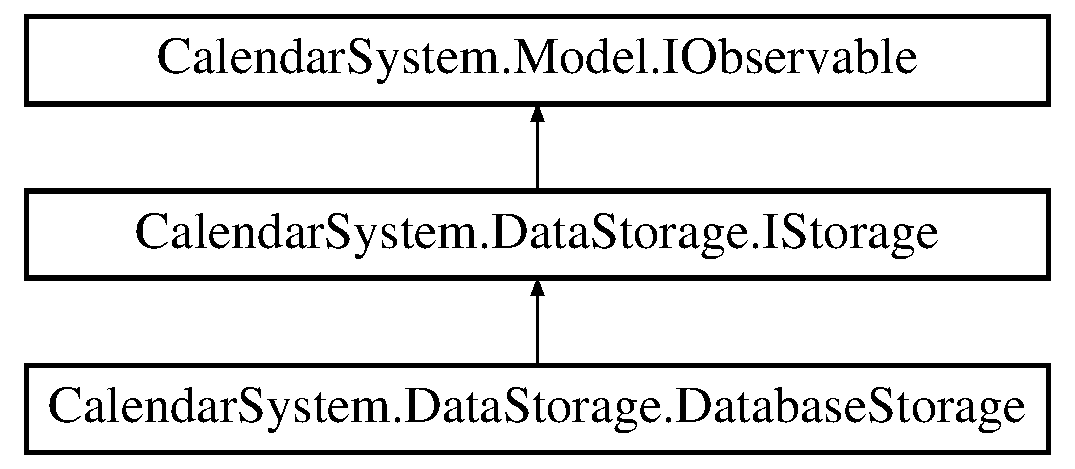
\includegraphics[height=3.000000cm]{class_calendar_system_1_1_data_storage_1_1_database_storage}
\end{center}
\end{figure}
\subsection*{Public Member Functions}
\begin{DoxyCompactItemize}
\item 
void \hyperlink{class_calendar_system_1_1_data_storage_1_1_database_storage_a3c7ccd413ae0f0d4684cf1b1998cddcd}{login\+Authentication} (string user\+Name, string password)
\begin{DoxyCompactList}\small\item\em Authenticate and download Calendar and events belonging to that user. \end{DoxyCompactList}\item 
void \hyperlink{class_calendar_system_1_1_data_storage_1_1_database_storage_ae4e6526f9d99e4a01b75a591a15fba9c}{Save\+Event} (string description, Date\+Time date\+Time, Time\+Span time\+Span, \hyperlink{class_calendar_system_1_1_model_1_1_notification}{Notification} notification)
\begin{DoxyCompactList}\small\item\em Save an event to the storage \end{DoxyCompactList}\item 
void \hyperlink{class_calendar_system_1_1_data_storage_1_1_database_storage_a9be31393f6b29a9b1b09297153da6b87}{Update\+Event} (int I\+D, string description, Date\+Time date\+Time, Time\+Span time\+Span, \hyperlink{class_calendar_system_1_1_model_1_1_notification}{Notification} notification)
\begin{DoxyCompactList}\small\item\em Update an event to the storage \end{DoxyCompactList}\item 
I\+List$<$ \hyperlink{interface_calendar_system_1_1_model_1_1_i_event}{I\+Event} $>$ \hyperlink{class_calendar_system_1_1_data_storage_1_1_database_storage_ab28e18e900a2011f271239952d9e2e26}{Get\+All\+Events} ()
\begin{DoxyCompactList}\small\item\em Returns all events in the active calendar \end{DoxyCompactList}\item 
\hyperlink{interface_calendar_system_1_1_model_1_1_i_event}{I\+Event} \hyperlink{class_calendar_system_1_1_data_storage_1_1_database_storage_a792702533aed5e26a856b216dffb67b4}{Get\+Event} (int I\+D)
\begin{DoxyCompactList}\small\item\em Get a single event with a given I\+D if possible. \end{DoxyCompactList}\item 
I\+List$<$ \hyperlink{interface_calendar_system_1_1_model_1_1_i_event}{I\+Event} $>$ \hyperlink{class_calendar_system_1_1_data_storage_1_1_database_storage_a168ecf83f6b5d8686fedd72c422b4486}{Get\+Events\+Between\+Dates} (Date\+Time begin\+Date\+Time, Date\+Time en\+Date\+Time)
\begin{DoxyCompactList}\small\item\em Return all events between to given dates. \end{DoxyCompactList}\item 
void \hyperlink{class_calendar_system_1_1_data_storage_1_1_database_storage_aee69c1fc20000371ee89ac06617d3610}{Create\+Tag} (\hyperlink{class_calendar_system_1_1_model_1_1_tag}{Tag} tag)
\begin{DoxyCompactList}\small\item\em Create a tag and save it in the storage. \end{DoxyCompactList}\item 
void \hyperlink{class_calendar_system_1_1_data_storage_1_1_database_storage_a9dde52dd67fc234b5f4ed217801968af}{Notify\+Observers} ()
\begin{DoxyCompactList}\small\item\em Notify observers that a change has happened. \end{DoxyCompactList}\item 
void \hyperlink{class_calendar_system_1_1_data_storage_1_1_database_storage_a6a80bdff8f3619508f20afdb3dddf650}{Be\+Observed} (\hyperlink{interface_calendar_system_1_1_model_1_1_i_observer}{I\+Observer} observer)
\begin{DoxyCompactList}\small\item\em Become observed by an object which class has implemented I\+Observer \end{DoxyCompactList}\item 
void \hyperlink{class_calendar_system_1_1_data_storage_1_1_database_storage_a21c41a45e85e0ace4e49838659587934}{Be\+Observed} (I\+List$<$ \hyperlink{interface_calendar_system_1_1_model_1_1_i_observer}{I\+Observer} $>$ observers)
\begin{DoxyCompactList}\small\item\em Be observed by a list of I\+Observer(s). \end{DoxyCompactList}\end{DoxyCompactItemize}


\subsection{Detailed Description}
A storage class which implements the \hyperlink{interface_calendar_system_1_1_data_storage_1_1_i_storage}{I\+Storage} interface. The class is meant to have a connection to a database where events will be added when they are created and put in the local Calendar class. 



\subsection{Member Function Documentation}
\hypertarget{class_calendar_system_1_1_data_storage_1_1_database_storage_a6a80bdff8f3619508f20afdb3dddf650}{\index{Calendar\+System\+::\+Data\+Storage\+::\+Database\+Storage@{Calendar\+System\+::\+Data\+Storage\+::\+Database\+Storage}!Be\+Observed@{Be\+Observed}}
\index{Be\+Observed@{Be\+Observed}!Calendar\+System\+::\+Data\+Storage\+::\+Database\+Storage@{Calendar\+System\+::\+Data\+Storage\+::\+Database\+Storage}}
\subsubsection[{Be\+Observed}]{\setlength{\rightskip}{0pt plus 5cm}void Calendar\+System.\+Data\+Storage.\+Database\+Storage.\+Be\+Observed (
\begin{DoxyParamCaption}
\item[{{\bf I\+Observer}}]{observer}
\end{DoxyParamCaption}
)}}\label{class_calendar_system_1_1_data_storage_1_1_database_storage_a6a80bdff8f3619508f20afdb3dddf650}


Become observed by an object which class has implemented I\+Observer 


\begin{DoxyParams}{Parameters}
{\em observer} & \\
\hline
\end{DoxyParams}


Implements \hyperlink{interface_calendar_system_1_1_model_1_1_i_observable_a23ca77451b9e6b19cdc111e0ef5f87c6}{Calendar\+System.\+Model.\+I\+Observable}.

\hypertarget{class_calendar_system_1_1_data_storage_1_1_database_storage_a21c41a45e85e0ace4e49838659587934}{\index{Calendar\+System\+::\+Data\+Storage\+::\+Database\+Storage@{Calendar\+System\+::\+Data\+Storage\+::\+Database\+Storage}!Be\+Observed@{Be\+Observed}}
\index{Be\+Observed@{Be\+Observed}!Calendar\+System\+::\+Data\+Storage\+::\+Database\+Storage@{Calendar\+System\+::\+Data\+Storage\+::\+Database\+Storage}}
\subsubsection[{Be\+Observed}]{\setlength{\rightskip}{0pt plus 5cm}void Calendar\+System.\+Data\+Storage.\+Database\+Storage.\+Be\+Observed (
\begin{DoxyParamCaption}
\item[{I\+List$<$ {\bf I\+Observer} $>$}]{observers}
\end{DoxyParamCaption}
)}}\label{class_calendar_system_1_1_data_storage_1_1_database_storage_a21c41a45e85e0ace4e49838659587934}


Be observed by a list of I\+Observer(s). 


\begin{DoxyParams}{Parameters}
{\em observers} & \\
\hline
\end{DoxyParams}


Implements \hyperlink{interface_calendar_system_1_1_model_1_1_i_observable_a53350aea0b6bf4ef1266d5d955db4700}{Calendar\+System.\+Model.\+I\+Observable}.

\hypertarget{class_calendar_system_1_1_data_storage_1_1_database_storage_aee69c1fc20000371ee89ac06617d3610}{\index{Calendar\+System\+::\+Data\+Storage\+::\+Database\+Storage@{Calendar\+System\+::\+Data\+Storage\+::\+Database\+Storage}!Create\+Tag@{Create\+Tag}}
\index{Create\+Tag@{Create\+Tag}!Calendar\+System\+::\+Data\+Storage\+::\+Database\+Storage@{Calendar\+System\+::\+Data\+Storage\+::\+Database\+Storage}}
\subsubsection[{Create\+Tag}]{\setlength{\rightskip}{0pt plus 5cm}void Calendar\+System.\+Data\+Storage.\+Database\+Storage.\+Create\+Tag (
\begin{DoxyParamCaption}
\item[{{\bf Tag}}]{tag}
\end{DoxyParamCaption}
)}}\label{class_calendar_system_1_1_data_storage_1_1_database_storage_aee69c1fc20000371ee89ac06617d3610}


Create a tag and save it in the storage. 


\begin{DoxyParams}{Parameters}
{\em tag} & \\
\hline
\end{DoxyParams}


Implements \hyperlink{interface_calendar_system_1_1_data_storage_1_1_i_storage_a8831822c54d654f17c98a8b13e679240}{Calendar\+System.\+Data\+Storage.\+I\+Storage}.

\hypertarget{class_calendar_system_1_1_data_storage_1_1_database_storage_ab28e18e900a2011f271239952d9e2e26}{\index{Calendar\+System\+::\+Data\+Storage\+::\+Database\+Storage@{Calendar\+System\+::\+Data\+Storage\+::\+Database\+Storage}!Get\+All\+Events@{Get\+All\+Events}}
\index{Get\+All\+Events@{Get\+All\+Events}!Calendar\+System\+::\+Data\+Storage\+::\+Database\+Storage@{Calendar\+System\+::\+Data\+Storage\+::\+Database\+Storage}}
\subsubsection[{Get\+All\+Events}]{\setlength{\rightskip}{0pt plus 5cm}I\+List$<${\bf I\+Event}$>$ Calendar\+System.\+Data\+Storage.\+Database\+Storage.\+Get\+All\+Events (
\begin{DoxyParamCaption}
{}
\end{DoxyParamCaption}
)}}\label{class_calendar_system_1_1_data_storage_1_1_database_storage_ab28e18e900a2011f271239952d9e2e26}


Returns all events in the active calendar 

\begin{DoxyReturn}{Returns}

\end{DoxyReturn}


Implements \hyperlink{interface_calendar_system_1_1_data_storage_1_1_i_storage_a06b5b139e4ef5fc7e66be8ffad9aed82}{Calendar\+System.\+Data\+Storage.\+I\+Storage}.

\hypertarget{class_calendar_system_1_1_data_storage_1_1_database_storage_a792702533aed5e26a856b216dffb67b4}{\index{Calendar\+System\+::\+Data\+Storage\+::\+Database\+Storage@{Calendar\+System\+::\+Data\+Storage\+::\+Database\+Storage}!Get\+Event@{Get\+Event}}
\index{Get\+Event@{Get\+Event}!Calendar\+System\+::\+Data\+Storage\+::\+Database\+Storage@{Calendar\+System\+::\+Data\+Storage\+::\+Database\+Storage}}
\subsubsection[{Get\+Event}]{\setlength{\rightskip}{0pt plus 5cm}{\bf I\+Event} Calendar\+System.\+Data\+Storage.\+Database\+Storage.\+Get\+Event (
\begin{DoxyParamCaption}
\item[{int}]{I\+D}
\end{DoxyParamCaption}
)}}\label{class_calendar_system_1_1_data_storage_1_1_database_storage_a792702533aed5e26a856b216dffb67b4}


Get a single event with a given I\+D if possible. 


\begin{DoxyParams}{Parameters}
{\em I\+D} & \\
\hline
\end{DoxyParams}
\begin{DoxyReturn}{Returns}

\end{DoxyReturn}


Implements \hyperlink{interface_calendar_system_1_1_data_storage_1_1_i_storage_a9b144e859410dbe90cc0876750c2872f}{Calendar\+System.\+Data\+Storage.\+I\+Storage}.

\hypertarget{class_calendar_system_1_1_data_storage_1_1_database_storage_a168ecf83f6b5d8686fedd72c422b4486}{\index{Calendar\+System\+::\+Data\+Storage\+::\+Database\+Storage@{Calendar\+System\+::\+Data\+Storage\+::\+Database\+Storage}!Get\+Events\+Between\+Dates@{Get\+Events\+Between\+Dates}}
\index{Get\+Events\+Between\+Dates@{Get\+Events\+Between\+Dates}!Calendar\+System\+::\+Data\+Storage\+::\+Database\+Storage@{Calendar\+System\+::\+Data\+Storage\+::\+Database\+Storage}}
\subsubsection[{Get\+Events\+Between\+Dates}]{\setlength{\rightskip}{0pt plus 5cm}I\+List$<${\bf I\+Event}$>$ Calendar\+System.\+Data\+Storage.\+Database\+Storage.\+Get\+Events\+Between\+Dates (
\begin{DoxyParamCaption}
\item[{Date\+Time}]{begin\+Date\+Time, }
\item[{Date\+Time}]{en\+Date\+Time}
\end{DoxyParamCaption}
)}}\label{class_calendar_system_1_1_data_storage_1_1_database_storage_a168ecf83f6b5d8686fedd72c422b4486}


Return all events between to given dates. 


\begin{DoxyParams}{Parameters}
{\em begin\+Date\+Time} & \\
\hline
{\em en\+Date\+Time} & \\
\hline
\end{DoxyParams}
\begin{DoxyReturn}{Returns}

\end{DoxyReturn}


Implements \hyperlink{interface_calendar_system_1_1_data_storage_1_1_i_storage_a1547353aae64841c1a79d60f07384c99}{Calendar\+System.\+Data\+Storage.\+I\+Storage}.

\hypertarget{class_calendar_system_1_1_data_storage_1_1_database_storage_a3c7ccd413ae0f0d4684cf1b1998cddcd}{\index{Calendar\+System\+::\+Data\+Storage\+::\+Database\+Storage@{Calendar\+System\+::\+Data\+Storage\+::\+Database\+Storage}!login\+Authentication@{login\+Authentication}}
\index{login\+Authentication@{login\+Authentication}!Calendar\+System\+::\+Data\+Storage\+::\+Database\+Storage@{Calendar\+System\+::\+Data\+Storage\+::\+Database\+Storage}}
\subsubsection[{login\+Authentication}]{\setlength{\rightskip}{0pt plus 5cm}void Calendar\+System.\+Data\+Storage.\+Database\+Storage.\+login\+Authentication (
\begin{DoxyParamCaption}
\item[{string}]{user\+Name, }
\item[{string}]{password}
\end{DoxyParamCaption}
)}}\label{class_calendar_system_1_1_data_storage_1_1_database_storage_a3c7ccd413ae0f0d4684cf1b1998cddcd}


Authenticate and download Calendar and events belonging to that user. 


\begin{DoxyParams}{Parameters}
{\em user\+Name} & \\
\hline
{\em password} & \\
\hline
\end{DoxyParams}
\begin{DoxyReturn}{Returns}

\end{DoxyReturn}


Implements \hyperlink{interface_calendar_system_1_1_data_storage_1_1_i_storage_a7818cf23c7f6dfca608c175d70558aa6}{Calendar\+System.\+Data\+Storage.\+I\+Storage}.

\hypertarget{class_calendar_system_1_1_data_storage_1_1_database_storage_a9dde52dd67fc234b5f4ed217801968af}{\index{Calendar\+System\+::\+Data\+Storage\+::\+Database\+Storage@{Calendar\+System\+::\+Data\+Storage\+::\+Database\+Storage}!Notify\+Observers@{Notify\+Observers}}
\index{Notify\+Observers@{Notify\+Observers}!Calendar\+System\+::\+Data\+Storage\+::\+Database\+Storage@{Calendar\+System\+::\+Data\+Storage\+::\+Database\+Storage}}
\subsubsection[{Notify\+Observers}]{\setlength{\rightskip}{0pt plus 5cm}void Calendar\+System.\+Data\+Storage.\+Database\+Storage.\+Notify\+Observers (
\begin{DoxyParamCaption}
{}
\end{DoxyParamCaption}
)}}\label{class_calendar_system_1_1_data_storage_1_1_database_storage_a9dde52dd67fc234b5f4ed217801968af}


Notify observers that a change has happened. 



Implements \hyperlink{interface_calendar_system_1_1_model_1_1_i_observable_aee5d17758abde1cd470266ede5fab0c1}{Calendar\+System.\+Model.\+I\+Observable}.

\hypertarget{class_calendar_system_1_1_data_storage_1_1_database_storage_ae4e6526f9d99e4a01b75a591a15fba9c}{\index{Calendar\+System\+::\+Data\+Storage\+::\+Database\+Storage@{Calendar\+System\+::\+Data\+Storage\+::\+Database\+Storage}!Save\+Event@{Save\+Event}}
\index{Save\+Event@{Save\+Event}!Calendar\+System\+::\+Data\+Storage\+::\+Database\+Storage@{Calendar\+System\+::\+Data\+Storage\+::\+Database\+Storage}}
\subsubsection[{Save\+Event}]{\setlength{\rightskip}{0pt plus 5cm}void Calendar\+System.\+Data\+Storage.\+Database\+Storage.\+Save\+Event (
\begin{DoxyParamCaption}
\item[{string}]{description, }
\item[{Date\+Time}]{date\+Time, }
\item[{Time\+Span}]{time\+Span, }
\item[{{\bf Notification}}]{notification}
\end{DoxyParamCaption}
)}}\label{class_calendar_system_1_1_data_storage_1_1_database_storage_ae4e6526f9d99e4a01b75a591a15fba9c}


Save an event to the storage 


\begin{DoxyParams}{Parameters}
{\em description} & \\
\hline
{\em date\+Time} & \\
\hline
{\em time\+Span} & \\
\hline
{\em notification} & \\
\hline
\end{DoxyParams}


Implements \hyperlink{interface_calendar_system_1_1_data_storage_1_1_i_storage_a041366475064bd7008e0546ac8d5d148}{Calendar\+System.\+Data\+Storage.\+I\+Storage}.

\hypertarget{class_calendar_system_1_1_data_storage_1_1_database_storage_a9be31393f6b29a9b1b09297153da6b87}{\index{Calendar\+System\+::\+Data\+Storage\+::\+Database\+Storage@{Calendar\+System\+::\+Data\+Storage\+::\+Database\+Storage}!Update\+Event@{Update\+Event}}
\index{Update\+Event@{Update\+Event}!Calendar\+System\+::\+Data\+Storage\+::\+Database\+Storage@{Calendar\+System\+::\+Data\+Storage\+::\+Database\+Storage}}
\subsubsection[{Update\+Event}]{\setlength{\rightskip}{0pt plus 5cm}void Calendar\+System.\+Data\+Storage.\+Database\+Storage.\+Update\+Event (
\begin{DoxyParamCaption}
\item[{int}]{I\+D, }
\item[{string}]{description, }
\item[{Date\+Time}]{date\+Time, }
\item[{Time\+Span}]{time\+Span, }
\item[{{\bf Notification}}]{notification}
\end{DoxyParamCaption}
)}}\label{class_calendar_system_1_1_data_storage_1_1_database_storage_a9be31393f6b29a9b1b09297153da6b87}


Update an event to the storage 


\begin{DoxyParams}{Parameters}
{\em description} & \\
\hline
{\em date\+Time} & \\
\hline
{\em time\+Span} & \\
\hline
{\em notification} & \\
\hline
\end{DoxyParams}


Implements \hyperlink{interface_calendar_system_1_1_data_storage_1_1_i_storage_a671ad7560e3d8197ec7867e98d3c138e}{Calendar\+System.\+Data\+Storage.\+I\+Storage}.



The documentation for this class was generated from the following file\+:\begin{DoxyCompactItemize}
\item 
Calendar\+System/\+Data\+Storage/Database\+Storage.\+cs\end{DoxyCompactItemize}

\hypertarget{class_calendar_system_1_1_model_1_1_event}{\section{Calendar\+System.\+Model.\+Event Class Reference}
\label{class_calendar_system_1_1_model_1_1_event}\index{Calendar\+System.\+Model.\+Event@{Calendar\+System.\+Model.\+Event}}
}


The event class implements the \hyperlink{interface_calendar_system_1_1_model_1_1_i_event}{I\+Event} interface and represents a period of time at a given time, with a couple of other fields.  


Inheritance diagram for Calendar\+System.\+Model.\+Event\+:\begin{figure}[H]
\begin{center}
\leavevmode
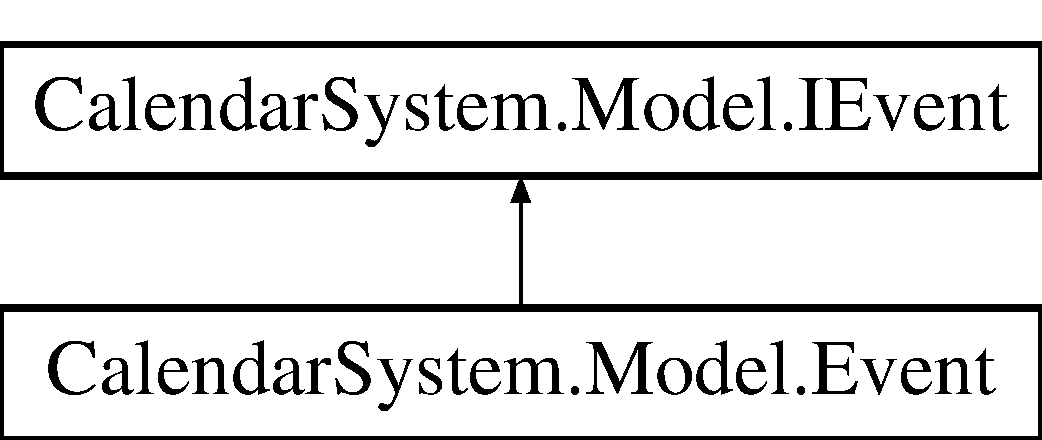
\includegraphics[height=2.000000cm]{class_calendar_system_1_1_model_1_1_event}
\end{center}
\end{figure}
\subsection*{Public Member Functions}
\begin{DoxyCompactItemize}
\item 
\hypertarget{class_calendar_system_1_1_model_1_1_event_a83bdd9e5882ea17cc8ccf8fa90b05267}{{\bfseries Event} (string description, Time\+Span timespan, Date\+Time date, \hyperlink{class_calendar_system_1_1_model_1_1_notification}{Notification} notification, int I\+D)}\label{class_calendar_system_1_1_model_1_1_event_a83bdd9e5882ea17cc8ccf8fa90b05267}

\item 
void \hyperlink{class_calendar_system_1_1_model_1_1_event_a3815e61cea5e1c94fe29ffcc103c1c6f}{change\+Tag} (\hyperlink{class_calendar_system_1_1_model_1_1_tag}{Tag} tag)
\begin{DoxyCompactList}\small\item\em Change the tag of the \end{DoxyCompactList}\end{DoxyCompactItemize}
\subsection*{Properties}
\begin{DoxyCompactItemize}
\item 
\hypertarget{class_calendar_system_1_1_model_1_1_event_a43e419d33262764a4147d4e082ebeeac}{\hyperlink{class_calendar_system_1_1_model_1_1_notification}{Notification} {\bfseries \+\_\+notification}\hspace{0.3cm}{\ttfamily  \mbox{[}get, set\mbox{]}}}\label{class_calendar_system_1_1_model_1_1_event_a43e419d33262764a4147d4e082ebeeac}

\item 
\hypertarget{class_calendar_system_1_1_model_1_1_event_a0533000133f17a13cbd98878e2972417}{Date\+Time {\bfseries \+\_\+date}\hspace{0.3cm}{\ttfamily  \mbox{[}get, set\mbox{]}}}\label{class_calendar_system_1_1_model_1_1_event_a0533000133f17a13cbd98878e2972417}

\item 
\hypertarget{class_calendar_system_1_1_model_1_1_event_a80a03074f9a64d1524a17580703f5b91}{Time\+Span {\bfseries \+\_\+time\+Span}\hspace{0.3cm}{\ttfamily  \mbox{[}get, set\mbox{]}}}\label{class_calendar_system_1_1_model_1_1_event_a80a03074f9a64d1524a17580703f5b91}

\item 
\hypertarget{class_calendar_system_1_1_model_1_1_event_ada1696e6a1810b53342a0a8cc413a65b}{string {\bfseries \+\_\+description}\hspace{0.3cm}{\ttfamily  \mbox{[}get, set\mbox{]}}}\label{class_calendar_system_1_1_model_1_1_event_ada1696e6a1810b53342a0a8cc413a65b}

\item 
\hypertarget{class_calendar_system_1_1_model_1_1_event_a7c5771b1fa4f3774ad2cff071dac03fe}{int {\bfseries \+\_\+\+I\+D}\hspace{0.3cm}{\ttfamily  \mbox{[}get\mbox{]}}}\label{class_calendar_system_1_1_model_1_1_event_a7c5771b1fa4f3774ad2cff071dac03fe}

\end{DoxyCompactItemize}


\subsection{Detailed Description}
The event class implements the \hyperlink{interface_calendar_system_1_1_model_1_1_i_event}{I\+Event} interface and represents a period of time at a given time, with a couple of other fields. 



\subsection{Member Function Documentation}
\hypertarget{class_calendar_system_1_1_model_1_1_event_a3815e61cea5e1c94fe29ffcc103c1c6f}{\index{Calendar\+System\+::\+Model\+::\+Event@{Calendar\+System\+::\+Model\+::\+Event}!change\+Tag@{change\+Tag}}
\index{change\+Tag@{change\+Tag}!Calendar\+System\+::\+Model\+::\+Event@{Calendar\+System\+::\+Model\+::\+Event}}
\subsubsection[{change\+Tag}]{\setlength{\rightskip}{0pt plus 5cm}void Calendar\+System.\+Model.\+Event.\+change\+Tag (
\begin{DoxyParamCaption}
\item[{{\bf Tag}}]{tag}
\end{DoxyParamCaption}
)}}\label{class_calendar_system_1_1_model_1_1_event_a3815e61cea5e1c94fe29ffcc103c1c6f}


Change the tag of the 


\begin{DoxyParams}{Parameters}
{\em tag} & \\
\hline
\end{DoxyParams}


Implements \hyperlink{interface_calendar_system_1_1_model_1_1_i_event}{Calendar\+System.\+Model.\+I\+Event}.



The documentation for this class was generated from the following file\+:\begin{DoxyCompactItemize}
\item 
Calendar\+System/\+Model/Event.\+cs\end{DoxyCompactItemize}

\hypertarget{class_calendar_system_1_1_view_1_1_event_view}{\section{Calendar\+System.\+View.\+Event\+View Class Reference}
\label{class_calendar_system_1_1_view_1_1_event_view}\index{Calendar\+System.\+View.\+Event\+View@{Calendar\+System.\+View.\+Event\+View}}
}


A class that visually represents an event object, or the creation thereof.  




\subsection{Detailed Description}
A class that visually represents an event object, or the creation thereof. 



The documentation for this class was generated from the following file\+:\begin{DoxyCompactItemize}
\item 
Calendar\+System/\+View/Event\+View.\+cs\end{DoxyCompactItemize}

\hypertarget{class_calendar_system_1_1_data_storage_1_1_fake_storage}{\section{Calendar\+System.\+Data\+Storage.\+Fake\+Storage Class Reference}
\label{class_calendar_system_1_1_data_storage_1_1_fake_storage}\index{Calendar\+System.\+Data\+Storage.\+Fake\+Storage@{Calendar\+System.\+Data\+Storage.\+Fake\+Storage}}
}


A storage class which implements the \hyperlink{interface_calendar_system_1_1_data_storage_1_1_i_storage}{I\+Storage} interface. The class is a fake storage in that sense that the fields and methods return components that are created at runtime. Therefore no events will be accessible from between runs of the system.  


Inheritance diagram for Calendar\+System.\+Data\+Storage.\+Fake\+Storage\+:\begin{figure}[H]
\begin{center}
\leavevmode
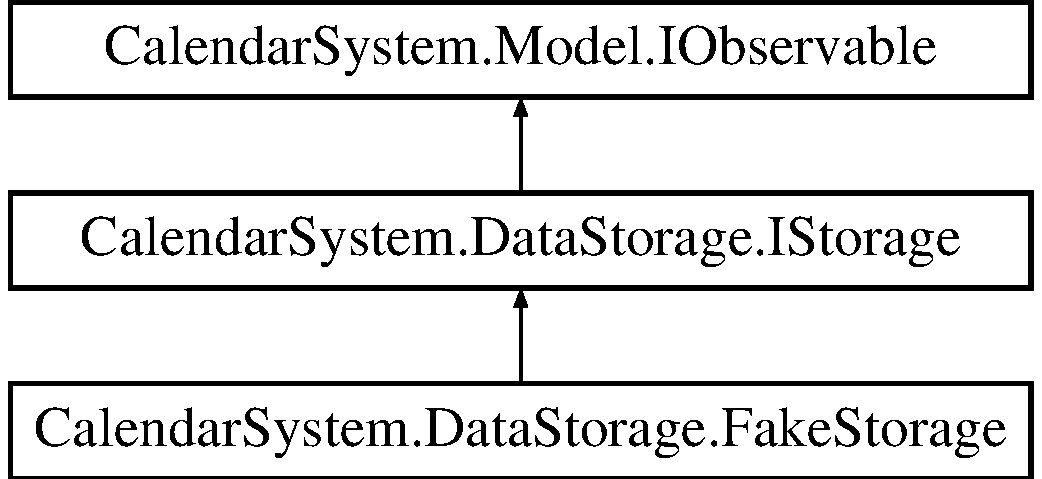
\includegraphics[height=3.000000cm]{class_calendar_system_1_1_data_storage_1_1_fake_storage}
\end{center}
\end{figure}
\subsection*{Public Member Functions}
\begin{DoxyCompactItemize}
\item 
void \hyperlink{class_calendar_system_1_1_data_storage_1_1_fake_storage_a589c203e56e50f0e71a1d202f7411a2f}{login\+Authentication} (string user\+Name, string password)
\begin{DoxyCompactList}\small\item\em Authenticate and download Calendar and events belonging to that user. \end{DoxyCompactList}\item 
void \hyperlink{class_calendar_system_1_1_data_storage_1_1_fake_storage_ac59fb43db4eb01c5b6153c7919608313}{Save\+Event} (string description, Date\+Time date\+Time, Time\+Span time\+Span, \hyperlink{class_calendar_system_1_1_model_1_1_notification}{Notification} notification)
\begin{DoxyCompactList}\small\item\em Save an event to the storage \end{DoxyCompactList}\item 
void \hyperlink{class_calendar_system_1_1_data_storage_1_1_fake_storage_a0d2bffbcf0485788321dbde8b419fc13}{Update\+Event} (int I\+D, string description, Date\+Time date\+Time, Time\+Span time\+Span, \hyperlink{class_calendar_system_1_1_model_1_1_notification}{Notification} notification)
\begin{DoxyCompactList}\small\item\em Update an event to the storage \end{DoxyCompactList}\item 
I\+List$<$ \hyperlink{interface_calendar_system_1_1_model_1_1_i_event}{I\+Event} $>$ \hyperlink{class_calendar_system_1_1_data_storage_1_1_fake_storage_a2b5d3fab2d4db84aa279e1408f56abb2}{Get\+All\+Events} ()
\begin{DoxyCompactList}\small\item\em Returns all events in the active calendar \end{DoxyCompactList}\item 
\hyperlink{interface_calendar_system_1_1_model_1_1_i_event}{I\+Event} \hyperlink{class_calendar_system_1_1_data_storage_1_1_fake_storage_a6f614104bbd16f6f04179dc6e7b41dd1}{Get\+Event} (int I\+D)
\begin{DoxyCompactList}\small\item\em Get a single event with a given I\+D if possible. \end{DoxyCompactList}\item 
I\+List$<$ \hyperlink{interface_calendar_system_1_1_model_1_1_i_event}{I\+Event} $>$ \hyperlink{class_calendar_system_1_1_data_storage_1_1_fake_storage_a16ce769932055ee3cc1bd47e945e7cfe}{Get\+Events\+Between\+Dates} (Date\+Time begin\+Date\+Time, Date\+Time en\+Date\+Time)
\begin{DoxyCompactList}\small\item\em Return all events between to given dates. \end{DoxyCompactList}\item 
void \hyperlink{class_calendar_system_1_1_data_storage_1_1_fake_storage_a713df02585d277ddb922d5912ad4a592}{Create\+Tag} (\hyperlink{class_calendar_system_1_1_model_1_1_tag}{Tag} tag)
\begin{DoxyCompactList}\small\item\em Create a tag and save it in the storage. \end{DoxyCompactList}\item 
void \hyperlink{class_calendar_system_1_1_data_storage_1_1_fake_storage_ad141dac914a11365efa50b8bf1bcc80d}{Notify\+Observers} ()
\begin{DoxyCompactList}\small\item\em Notify observers that a change has happened. \end{DoxyCompactList}\item 
void \hyperlink{class_calendar_system_1_1_data_storage_1_1_fake_storage_a145d71dfbca477a39bbd5c865f2e10fe}{Be\+Observed} (\hyperlink{interface_calendar_system_1_1_model_1_1_i_observer}{I\+Observer} observer)
\begin{DoxyCompactList}\small\item\em Become observed by an object which class has implemented I\+Observer \end{DoxyCompactList}\item 
void \hyperlink{class_calendar_system_1_1_data_storage_1_1_fake_storage_ab9861bbbb0b5f5af8928f4c7efec59b5}{Be\+Observed} (I\+List$<$ \hyperlink{interface_calendar_system_1_1_model_1_1_i_observer}{I\+Observer} $>$ observers)
\begin{DoxyCompactList}\small\item\em Be observed by a list of I\+Observer(s). \end{DoxyCompactList}\end{DoxyCompactItemize}


\subsection{Detailed Description}
A storage class which implements the \hyperlink{interface_calendar_system_1_1_data_storage_1_1_i_storage}{I\+Storage} interface. The class is a fake storage in that sense that the fields and methods return components that are created at runtime. Therefore no events will be accessible from between runs of the system. 



\subsection{Member Function Documentation}
\hypertarget{class_calendar_system_1_1_data_storage_1_1_fake_storage_a145d71dfbca477a39bbd5c865f2e10fe}{\index{Calendar\+System\+::\+Data\+Storage\+::\+Fake\+Storage@{Calendar\+System\+::\+Data\+Storage\+::\+Fake\+Storage}!Be\+Observed@{Be\+Observed}}
\index{Be\+Observed@{Be\+Observed}!Calendar\+System\+::\+Data\+Storage\+::\+Fake\+Storage@{Calendar\+System\+::\+Data\+Storage\+::\+Fake\+Storage}}
\subsubsection[{Be\+Observed}]{\setlength{\rightskip}{0pt plus 5cm}void Calendar\+System.\+Data\+Storage.\+Fake\+Storage.\+Be\+Observed (
\begin{DoxyParamCaption}
\item[{{\bf I\+Observer}}]{observer}
\end{DoxyParamCaption}
)}}\label{class_calendar_system_1_1_data_storage_1_1_fake_storage_a145d71dfbca477a39bbd5c865f2e10fe}


Become observed by an object which class has implemented I\+Observer 


\begin{DoxyParams}{Parameters}
{\em observer} & \\
\hline
\end{DoxyParams}


Implements \hyperlink{interface_calendar_system_1_1_model_1_1_i_observable_a23ca77451b9e6b19cdc111e0ef5f87c6}{Calendar\+System.\+Model.\+I\+Observable}.

\hypertarget{class_calendar_system_1_1_data_storage_1_1_fake_storage_ab9861bbbb0b5f5af8928f4c7efec59b5}{\index{Calendar\+System\+::\+Data\+Storage\+::\+Fake\+Storage@{Calendar\+System\+::\+Data\+Storage\+::\+Fake\+Storage}!Be\+Observed@{Be\+Observed}}
\index{Be\+Observed@{Be\+Observed}!Calendar\+System\+::\+Data\+Storage\+::\+Fake\+Storage@{Calendar\+System\+::\+Data\+Storage\+::\+Fake\+Storage}}
\subsubsection[{Be\+Observed}]{\setlength{\rightskip}{0pt plus 5cm}void Calendar\+System.\+Data\+Storage.\+Fake\+Storage.\+Be\+Observed (
\begin{DoxyParamCaption}
\item[{I\+List$<$ {\bf I\+Observer} $>$}]{observers}
\end{DoxyParamCaption}
)}}\label{class_calendar_system_1_1_data_storage_1_1_fake_storage_ab9861bbbb0b5f5af8928f4c7efec59b5}


Be observed by a list of I\+Observer(s). 


\begin{DoxyParams}{Parameters}
{\em observers} & \\
\hline
\end{DoxyParams}


Implements \hyperlink{interface_calendar_system_1_1_model_1_1_i_observable_a53350aea0b6bf4ef1266d5d955db4700}{Calendar\+System.\+Model.\+I\+Observable}.

\hypertarget{class_calendar_system_1_1_data_storage_1_1_fake_storage_a713df02585d277ddb922d5912ad4a592}{\index{Calendar\+System\+::\+Data\+Storage\+::\+Fake\+Storage@{Calendar\+System\+::\+Data\+Storage\+::\+Fake\+Storage}!Create\+Tag@{Create\+Tag}}
\index{Create\+Tag@{Create\+Tag}!Calendar\+System\+::\+Data\+Storage\+::\+Fake\+Storage@{Calendar\+System\+::\+Data\+Storage\+::\+Fake\+Storage}}
\subsubsection[{Create\+Tag}]{\setlength{\rightskip}{0pt plus 5cm}void Calendar\+System.\+Data\+Storage.\+Fake\+Storage.\+Create\+Tag (
\begin{DoxyParamCaption}
\item[{{\bf Tag}}]{tag}
\end{DoxyParamCaption}
)}}\label{class_calendar_system_1_1_data_storage_1_1_fake_storage_a713df02585d277ddb922d5912ad4a592}


Create a tag and save it in the storage. 


\begin{DoxyParams}{Parameters}
{\em tag} & \\
\hline
\end{DoxyParams}


Implements \hyperlink{interface_calendar_system_1_1_data_storage_1_1_i_storage_a8831822c54d654f17c98a8b13e679240}{Calendar\+System.\+Data\+Storage.\+I\+Storage}.

\hypertarget{class_calendar_system_1_1_data_storage_1_1_fake_storage_a2b5d3fab2d4db84aa279e1408f56abb2}{\index{Calendar\+System\+::\+Data\+Storage\+::\+Fake\+Storage@{Calendar\+System\+::\+Data\+Storage\+::\+Fake\+Storage}!Get\+All\+Events@{Get\+All\+Events}}
\index{Get\+All\+Events@{Get\+All\+Events}!Calendar\+System\+::\+Data\+Storage\+::\+Fake\+Storage@{Calendar\+System\+::\+Data\+Storage\+::\+Fake\+Storage}}
\subsubsection[{Get\+All\+Events}]{\setlength{\rightskip}{0pt plus 5cm}I\+List$<${\bf I\+Event}$>$ Calendar\+System.\+Data\+Storage.\+Fake\+Storage.\+Get\+All\+Events (
\begin{DoxyParamCaption}
{}
\end{DoxyParamCaption}
)}}\label{class_calendar_system_1_1_data_storage_1_1_fake_storage_a2b5d3fab2d4db84aa279e1408f56abb2}


Returns all events in the active calendar 

\begin{DoxyReturn}{Returns}

\end{DoxyReturn}


Implements \hyperlink{interface_calendar_system_1_1_data_storage_1_1_i_storage_a06b5b139e4ef5fc7e66be8ffad9aed82}{Calendar\+System.\+Data\+Storage.\+I\+Storage}.

\hypertarget{class_calendar_system_1_1_data_storage_1_1_fake_storage_a6f614104bbd16f6f04179dc6e7b41dd1}{\index{Calendar\+System\+::\+Data\+Storage\+::\+Fake\+Storage@{Calendar\+System\+::\+Data\+Storage\+::\+Fake\+Storage}!Get\+Event@{Get\+Event}}
\index{Get\+Event@{Get\+Event}!Calendar\+System\+::\+Data\+Storage\+::\+Fake\+Storage@{Calendar\+System\+::\+Data\+Storage\+::\+Fake\+Storage}}
\subsubsection[{Get\+Event}]{\setlength{\rightskip}{0pt plus 5cm}{\bf I\+Event} Calendar\+System.\+Data\+Storage.\+Fake\+Storage.\+Get\+Event (
\begin{DoxyParamCaption}
\item[{int}]{I\+D}
\end{DoxyParamCaption}
)}}\label{class_calendar_system_1_1_data_storage_1_1_fake_storage_a6f614104bbd16f6f04179dc6e7b41dd1}


Get a single event with a given I\+D if possible. 


\begin{DoxyParams}{Parameters}
{\em I\+D} & \\
\hline
\end{DoxyParams}
\begin{DoxyReturn}{Returns}

\end{DoxyReturn}


Implements \hyperlink{interface_calendar_system_1_1_data_storage_1_1_i_storage_a9b144e859410dbe90cc0876750c2872f}{Calendar\+System.\+Data\+Storage.\+I\+Storage}.

\hypertarget{class_calendar_system_1_1_data_storage_1_1_fake_storage_a16ce769932055ee3cc1bd47e945e7cfe}{\index{Calendar\+System\+::\+Data\+Storage\+::\+Fake\+Storage@{Calendar\+System\+::\+Data\+Storage\+::\+Fake\+Storage}!Get\+Events\+Between\+Dates@{Get\+Events\+Between\+Dates}}
\index{Get\+Events\+Between\+Dates@{Get\+Events\+Between\+Dates}!Calendar\+System\+::\+Data\+Storage\+::\+Fake\+Storage@{Calendar\+System\+::\+Data\+Storage\+::\+Fake\+Storage}}
\subsubsection[{Get\+Events\+Between\+Dates}]{\setlength{\rightskip}{0pt plus 5cm}I\+List$<${\bf I\+Event}$>$ Calendar\+System.\+Data\+Storage.\+Fake\+Storage.\+Get\+Events\+Between\+Dates (
\begin{DoxyParamCaption}
\item[{Date\+Time}]{begin\+Date\+Time, }
\item[{Date\+Time}]{en\+Date\+Time}
\end{DoxyParamCaption}
)}}\label{class_calendar_system_1_1_data_storage_1_1_fake_storage_a16ce769932055ee3cc1bd47e945e7cfe}


Return all events between to given dates. 


\begin{DoxyParams}{Parameters}
{\em begin\+Date\+Time} & \\
\hline
{\em en\+Date\+Time} & \\
\hline
\end{DoxyParams}
\begin{DoxyReturn}{Returns}

\end{DoxyReturn}


Implements \hyperlink{interface_calendar_system_1_1_data_storage_1_1_i_storage_a1547353aae64841c1a79d60f07384c99}{Calendar\+System.\+Data\+Storage.\+I\+Storage}.

\hypertarget{class_calendar_system_1_1_data_storage_1_1_fake_storage_a589c203e56e50f0e71a1d202f7411a2f}{\index{Calendar\+System\+::\+Data\+Storage\+::\+Fake\+Storage@{Calendar\+System\+::\+Data\+Storage\+::\+Fake\+Storage}!login\+Authentication@{login\+Authentication}}
\index{login\+Authentication@{login\+Authentication}!Calendar\+System\+::\+Data\+Storage\+::\+Fake\+Storage@{Calendar\+System\+::\+Data\+Storage\+::\+Fake\+Storage}}
\subsubsection[{login\+Authentication}]{\setlength{\rightskip}{0pt plus 5cm}void Calendar\+System.\+Data\+Storage.\+Fake\+Storage.\+login\+Authentication (
\begin{DoxyParamCaption}
\item[{string}]{user\+Name, }
\item[{string}]{password}
\end{DoxyParamCaption}
)}}\label{class_calendar_system_1_1_data_storage_1_1_fake_storage_a589c203e56e50f0e71a1d202f7411a2f}


Authenticate and download Calendar and events belonging to that user. 


\begin{DoxyParams}{Parameters}
{\em user\+Name} & \\
\hline
{\em password} & \\
\hline
\end{DoxyParams}
\begin{DoxyReturn}{Returns}

\end{DoxyReturn}


Implements \hyperlink{interface_calendar_system_1_1_data_storage_1_1_i_storage_a7818cf23c7f6dfca608c175d70558aa6}{Calendar\+System.\+Data\+Storage.\+I\+Storage}.

\hypertarget{class_calendar_system_1_1_data_storage_1_1_fake_storage_ad141dac914a11365efa50b8bf1bcc80d}{\index{Calendar\+System\+::\+Data\+Storage\+::\+Fake\+Storage@{Calendar\+System\+::\+Data\+Storage\+::\+Fake\+Storage}!Notify\+Observers@{Notify\+Observers}}
\index{Notify\+Observers@{Notify\+Observers}!Calendar\+System\+::\+Data\+Storage\+::\+Fake\+Storage@{Calendar\+System\+::\+Data\+Storage\+::\+Fake\+Storage}}
\subsubsection[{Notify\+Observers}]{\setlength{\rightskip}{0pt plus 5cm}void Calendar\+System.\+Data\+Storage.\+Fake\+Storage.\+Notify\+Observers (
\begin{DoxyParamCaption}
{}
\end{DoxyParamCaption}
)}}\label{class_calendar_system_1_1_data_storage_1_1_fake_storage_ad141dac914a11365efa50b8bf1bcc80d}


Notify observers that a change has happened. 



Implements \hyperlink{interface_calendar_system_1_1_model_1_1_i_observable_aee5d17758abde1cd470266ede5fab0c1}{Calendar\+System.\+Model.\+I\+Observable}.

\hypertarget{class_calendar_system_1_1_data_storage_1_1_fake_storage_ac59fb43db4eb01c5b6153c7919608313}{\index{Calendar\+System\+::\+Data\+Storage\+::\+Fake\+Storage@{Calendar\+System\+::\+Data\+Storage\+::\+Fake\+Storage}!Save\+Event@{Save\+Event}}
\index{Save\+Event@{Save\+Event}!Calendar\+System\+::\+Data\+Storage\+::\+Fake\+Storage@{Calendar\+System\+::\+Data\+Storage\+::\+Fake\+Storage}}
\subsubsection[{Save\+Event}]{\setlength{\rightskip}{0pt plus 5cm}void Calendar\+System.\+Data\+Storage.\+Fake\+Storage.\+Save\+Event (
\begin{DoxyParamCaption}
\item[{string}]{description, }
\item[{Date\+Time}]{date\+Time, }
\item[{Time\+Span}]{time\+Span, }
\item[{{\bf Notification}}]{notification}
\end{DoxyParamCaption}
)}}\label{class_calendar_system_1_1_data_storage_1_1_fake_storage_ac59fb43db4eb01c5b6153c7919608313}


Save an event to the storage 


\begin{DoxyParams}{Parameters}
{\em description} & \\
\hline
{\em date\+Time} & \\
\hline
{\em time\+Span} & \\
\hline
{\em notification} & \\
\hline
\end{DoxyParams}


Implements \hyperlink{interface_calendar_system_1_1_data_storage_1_1_i_storage_a041366475064bd7008e0546ac8d5d148}{Calendar\+System.\+Data\+Storage.\+I\+Storage}.

\hypertarget{class_calendar_system_1_1_data_storage_1_1_fake_storage_a0d2bffbcf0485788321dbde8b419fc13}{\index{Calendar\+System\+::\+Data\+Storage\+::\+Fake\+Storage@{Calendar\+System\+::\+Data\+Storage\+::\+Fake\+Storage}!Update\+Event@{Update\+Event}}
\index{Update\+Event@{Update\+Event}!Calendar\+System\+::\+Data\+Storage\+::\+Fake\+Storage@{Calendar\+System\+::\+Data\+Storage\+::\+Fake\+Storage}}
\subsubsection[{Update\+Event}]{\setlength{\rightskip}{0pt plus 5cm}void Calendar\+System.\+Data\+Storage.\+Fake\+Storage.\+Update\+Event (
\begin{DoxyParamCaption}
\item[{int}]{I\+D, }
\item[{string}]{description, }
\item[{Date\+Time}]{date\+Time, }
\item[{Time\+Span}]{time\+Span, }
\item[{{\bf Notification}}]{notification}
\end{DoxyParamCaption}
)}}\label{class_calendar_system_1_1_data_storage_1_1_fake_storage_a0d2bffbcf0485788321dbde8b419fc13}


Update an event to the storage 


\begin{DoxyParams}{Parameters}
{\em description} & \\
\hline
{\em date\+Time} & \\
\hline
{\em time\+Span} & \\
\hline
{\em notification} & \\
\hline
\end{DoxyParams}


Implements \hyperlink{interface_calendar_system_1_1_data_storage_1_1_i_storage_a671ad7560e3d8197ec7867e98d3c138e}{Calendar\+System.\+Data\+Storage.\+I\+Storage}.



The documentation for this class was generated from the following file\+:\begin{DoxyCompactItemize}
\item 
Calendar\+System/\+Data\+Storage/Fake\+Storage.\+cs\end{DoxyCompactItemize}

\hypertarget{interface_calendar_system_1_1_model_1_1_i_event}{\section{Calendar\+System.\+Model.\+I\+Event Interface Reference}
\label{interface_calendar_system_1_1_model_1_1_i_event}\index{Calendar\+System.\+Model.\+I\+Event@{Calendar\+System.\+Model.\+I\+Event}}
}


An interface for event classes, used for given the minimum an event class must be able to do, and have.  


Inheritance diagram for Calendar\+System.\+Model.\+I\+Event\+:\begin{figure}[H]
\begin{center}
\leavevmode
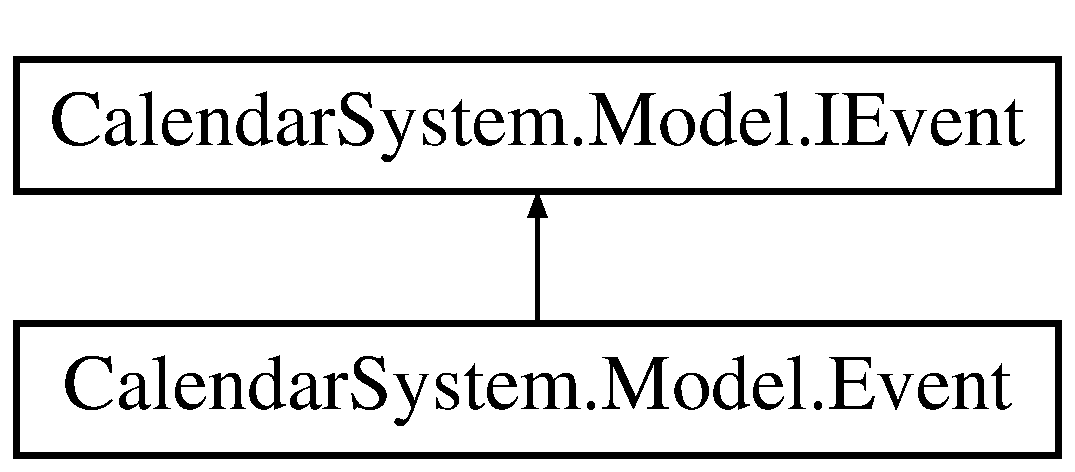
\includegraphics[height=2.000000cm]{interface_calendar_system_1_1_model_1_1_i_event}
\end{center}
\end{figure}
\subsection*{Public Member Functions}
\begin{DoxyCompactItemize}
\item 
\hypertarget{interface_calendar_system_1_1_model_1_1_i_event_a6a455d39dad509964a5f641980f248dd}{void {\bfseries change\+Tag} (\hyperlink{class_calendar_system_1_1_model_1_1_tag}{Tag} tag)}\label{interface_calendar_system_1_1_model_1_1_i_event_a6a455d39dad509964a5f641980f248dd}

\end{DoxyCompactItemize}
\subsection*{Properties}
\begin{DoxyCompactItemize}
\item 
\hypertarget{interface_calendar_system_1_1_model_1_1_i_event_a9fa4752d2b8e05d79b70951b46cb1d7a}{\hyperlink{class_calendar_system_1_1_model_1_1_notification}{Notification} {\bfseries \+\_\+notification}\hspace{0.3cm}{\ttfamily  \mbox{[}get, set\mbox{]}}}\label{interface_calendar_system_1_1_model_1_1_i_event_a9fa4752d2b8e05d79b70951b46cb1d7a}

\item 
\hypertarget{interface_calendar_system_1_1_model_1_1_i_event_a0c3e5af1e6f4c3fc5878677b0a37dc60}{Date\+Time {\bfseries \+\_\+date}\hspace{0.3cm}{\ttfamily  \mbox{[}get, set\mbox{]}}}\label{interface_calendar_system_1_1_model_1_1_i_event_a0c3e5af1e6f4c3fc5878677b0a37dc60}

\item 
\hypertarget{interface_calendar_system_1_1_model_1_1_i_event_a8bc4cc2289f2e187753374309e9e905e}{Time\+Span {\bfseries \+\_\+time\+Span}\hspace{0.3cm}{\ttfamily  \mbox{[}get, set\mbox{]}}}\label{interface_calendar_system_1_1_model_1_1_i_event_a8bc4cc2289f2e187753374309e9e905e}

\item 
\hypertarget{interface_calendar_system_1_1_model_1_1_i_event_a8a59754858a0ce6943d6a21471566cee}{string {\bfseries \+\_\+description}\hspace{0.3cm}{\ttfamily  \mbox{[}get, set\mbox{]}}}\label{interface_calendar_system_1_1_model_1_1_i_event_a8a59754858a0ce6943d6a21471566cee}

\item 
\hypertarget{interface_calendar_system_1_1_model_1_1_i_event_a48d61475d0de8c5a6b925057cdfeb1bd}{int {\bfseries \+\_\+\+I\+D}\hspace{0.3cm}{\ttfamily  \mbox{[}get\mbox{]}}}\label{interface_calendar_system_1_1_model_1_1_i_event_a48d61475d0de8c5a6b925057cdfeb1bd}

\end{DoxyCompactItemize}


\subsection{Detailed Description}
An interface for event classes, used for given the minimum an event class must be able to do, and have. 



The documentation for this interface was generated from the following file\+:\begin{DoxyCompactItemize}
\item 
Calendar\+System/\+Model/I\+Event.\+cs\end{DoxyCompactItemize}

\hypertarget{class_calendar_system_1_1_controller_1_1_input_controller}{\section{Calendar\+System.\+Controller.\+Input\+Controller Class Reference}
\label{class_calendar_system_1_1_controller_1_1_input_controller}\index{Calendar\+System.\+Controller.\+Input\+Controller@{Calendar\+System.\+Controller.\+Input\+Controller}}
}


The inputcontroller handles all incoming user interaction, such as button presses and so on.  


\subsection*{Public Member Functions}
\begin{DoxyCompactItemize}
\item 
void \hyperlink{class_calendar_system_1_1_controller_1_1_input_controller_a6a6b437e915b97c6ca03b846baeffbef}{Create\+Calendar\+Entry} (string description, int year, int month, int day, int start\+Hour, int end\+Hour)
\begin{DoxyCompactList}\small\item\em A method which will often be called from the view. The method takes some parameters and gives the to the storage, where an event will be created and uploaded. \end{DoxyCompactList}\item 
void \hyperlink{class_calendar_system_1_1_controller_1_1_input_controller_a600a42ef535df171f500022244b7d432}{Update\+Calendar\+Entry} (int I\+D, string description, int year, int month, int day, int start\+Hour, int end\+Hour)
\begin{DoxyCompactList}\small\item\em A method which will often be called from the view. The method takes some parameters and gives the to the storage, where an event will be updated and uploaded. \end{DoxyCompactList}\item 
void \hyperlink{class_calendar_system_1_1_controller_1_1_input_controller_ab7b792da94ca5d8cfffacb501c97be0c}{Create\+Tag} (string new\+Tag)
\begin{DoxyCompactList}\small\item\em A method to create a tag and put it in the datastorage \end{DoxyCompactList}\item 
void \hyperlink{class_calendar_system_1_1_controller_1_1_input_controller_aaf0f1ccecfd2ba1d09759d4d58b39f34}{Change\+Overview\+Type} (string overview\+Type)
\begin{DoxyCompactList}\small\item\em Send the request for a new view type to the view\+Controller. \end{DoxyCompactList}\end{DoxyCompactItemize}
\subsection*{Static Public Member Functions}
\begin{DoxyCompactItemize}
\item 
static \hyperlink{class_calendar_system_1_1_controller_1_1_input_controller}{Input\+Controller} \hyperlink{class_calendar_system_1_1_controller_1_1_input_controller_ac2ab91bd66d05a5bb762ede338dabc47}{get\+Instance} ()
\begin{DoxyCompactList}\small\item\em Singleton pattern. Makes sure only one instance can exist at a given time, and give classes easy access to the controller. \end{DoxyCompactList}\end{DoxyCompactItemize}
\subsection*{Properties}
\begin{DoxyCompactItemize}
\item 
\hypertarget{class_calendar_system_1_1_controller_1_1_input_controller_a9a599456b056daf9a5b5dc47bc385c78}{\hyperlink{interface_calendar_system_1_1_data_storage_1_1_i_storage}{I\+Storage} {\bfseries \+\_\+storage}\hspace{0.3cm}{\ttfamily  \mbox{[}get\mbox{]}}}\label{class_calendar_system_1_1_controller_1_1_input_controller_a9a599456b056daf9a5b5dc47bc385c78}

\end{DoxyCompactItemize}


\subsection{Detailed Description}
The inputcontroller handles all incoming user interaction, such as button presses and so on. 



\subsection{Member Function Documentation}
\hypertarget{class_calendar_system_1_1_controller_1_1_input_controller_aaf0f1ccecfd2ba1d09759d4d58b39f34}{\index{Calendar\+System\+::\+Controller\+::\+Input\+Controller@{Calendar\+System\+::\+Controller\+::\+Input\+Controller}!Change\+Overview\+Type@{Change\+Overview\+Type}}
\index{Change\+Overview\+Type@{Change\+Overview\+Type}!Calendar\+System\+::\+Controller\+::\+Input\+Controller@{Calendar\+System\+::\+Controller\+::\+Input\+Controller}}
\subsubsection[{Change\+Overview\+Type}]{\setlength{\rightskip}{0pt plus 5cm}void Calendar\+System.\+Controller.\+Input\+Controller.\+Change\+Overview\+Type (
\begin{DoxyParamCaption}
\item[{string}]{overview\+Type}
\end{DoxyParamCaption}
)}}\label{class_calendar_system_1_1_controller_1_1_input_controller_aaf0f1ccecfd2ba1d09759d4d58b39f34}


Send the request for a new view type to the view\+Controller. 


\begin{DoxyParams}{Parameters}
{\em overview\+Type} & A string which represents a overview type\\
\hline
\end{DoxyParams}
\hypertarget{class_calendar_system_1_1_controller_1_1_input_controller_a6a6b437e915b97c6ca03b846baeffbef}{\index{Calendar\+System\+::\+Controller\+::\+Input\+Controller@{Calendar\+System\+::\+Controller\+::\+Input\+Controller}!Create\+Calendar\+Entry@{Create\+Calendar\+Entry}}
\index{Create\+Calendar\+Entry@{Create\+Calendar\+Entry}!Calendar\+System\+::\+Controller\+::\+Input\+Controller@{Calendar\+System\+::\+Controller\+::\+Input\+Controller}}
\subsubsection[{Create\+Calendar\+Entry}]{\setlength{\rightskip}{0pt plus 5cm}void Calendar\+System.\+Controller.\+Input\+Controller.\+Create\+Calendar\+Entry (
\begin{DoxyParamCaption}
\item[{string}]{description, }
\item[{int}]{year, }
\item[{int}]{month, }
\item[{int}]{day, }
\item[{int}]{start\+Hour, }
\item[{int}]{end\+Hour}
\end{DoxyParamCaption}
)}}\label{class_calendar_system_1_1_controller_1_1_input_controller_a6a6b437e915b97c6ca03b846baeffbef}


A method which will often be called from the view. The method takes some parameters and gives the to the storage, where an event will be created and uploaded. 


\begin{DoxyParams}{Parameters}
{\em description} & The description of an event\\
\hline
{\em month} & The month of the event\\
\hline
{\em day} & The day of the event\\
\hline
{\em start\+Hour} & The start hour of the event\\
\hline
{\em end\+Hour} & The end hour of the event\\
\hline
\end{DoxyParams}
\hypertarget{class_calendar_system_1_1_controller_1_1_input_controller_ab7b792da94ca5d8cfffacb501c97be0c}{\index{Calendar\+System\+::\+Controller\+::\+Input\+Controller@{Calendar\+System\+::\+Controller\+::\+Input\+Controller}!Create\+Tag@{Create\+Tag}}
\index{Create\+Tag@{Create\+Tag}!Calendar\+System\+::\+Controller\+::\+Input\+Controller@{Calendar\+System\+::\+Controller\+::\+Input\+Controller}}
\subsubsection[{Create\+Tag}]{\setlength{\rightskip}{0pt plus 5cm}void Calendar\+System.\+Controller.\+Input\+Controller.\+Create\+Tag (
\begin{DoxyParamCaption}
\item[{string}]{new\+Tag}
\end{DoxyParamCaption}
)}}\label{class_calendar_system_1_1_controller_1_1_input_controller_ab7b792da94ca5d8cfffacb501c97be0c}


A method to create a tag and put it in the datastorage 


\begin{DoxyParams}{Parameters}
{\em new\+Tag} & \\
\hline
\end{DoxyParams}
\hypertarget{class_calendar_system_1_1_controller_1_1_input_controller_ac2ab91bd66d05a5bb762ede338dabc47}{\index{Calendar\+System\+::\+Controller\+::\+Input\+Controller@{Calendar\+System\+::\+Controller\+::\+Input\+Controller}!get\+Instance@{get\+Instance}}
\index{get\+Instance@{get\+Instance}!Calendar\+System\+::\+Controller\+::\+Input\+Controller@{Calendar\+System\+::\+Controller\+::\+Input\+Controller}}
\subsubsection[{get\+Instance}]{\setlength{\rightskip}{0pt plus 5cm}static {\bf Input\+Controller} Calendar\+System.\+Controller.\+Input\+Controller.\+get\+Instance (
\begin{DoxyParamCaption}
{}
\end{DoxyParamCaption}
)\hspace{0.3cm}{\ttfamily [static]}}}\label{class_calendar_system_1_1_controller_1_1_input_controller_ac2ab91bd66d05a5bb762ede338dabc47}


Singleton pattern. Makes sure only one instance can exist at a given time, and give classes easy access to the controller. 

\begin{DoxyReturn}{Returns}
The only instance of the class
\end{DoxyReturn}
\hypertarget{class_calendar_system_1_1_controller_1_1_input_controller_a600a42ef535df171f500022244b7d432}{\index{Calendar\+System\+::\+Controller\+::\+Input\+Controller@{Calendar\+System\+::\+Controller\+::\+Input\+Controller}!Update\+Calendar\+Entry@{Update\+Calendar\+Entry}}
\index{Update\+Calendar\+Entry@{Update\+Calendar\+Entry}!Calendar\+System\+::\+Controller\+::\+Input\+Controller@{Calendar\+System\+::\+Controller\+::\+Input\+Controller}}
\subsubsection[{Update\+Calendar\+Entry}]{\setlength{\rightskip}{0pt plus 5cm}void Calendar\+System.\+Controller.\+Input\+Controller.\+Update\+Calendar\+Entry (
\begin{DoxyParamCaption}
\item[{int}]{I\+D, }
\item[{string}]{description, }
\item[{int}]{year, }
\item[{int}]{month, }
\item[{int}]{day, }
\item[{int}]{start\+Hour, }
\item[{int}]{end\+Hour}
\end{DoxyParamCaption}
)}}\label{class_calendar_system_1_1_controller_1_1_input_controller_a600a42ef535df171f500022244b7d432}


A method which will often be called from the view. The method takes some parameters and gives the to the storage, where an event will be updated and uploaded. 


\begin{DoxyParams}{Parameters}
{\em I\+D} & The I\+D of the \\
\hline
{\em description} & The description of an event\\
\hline
{\em month} & The month of the event\\
\hline
{\em day} & The day of the event\\
\hline
{\em start\+Hour} & The start hour of the event\\
\hline
{\em end\+Hour} & The end hour of the event\\
\hline
\end{DoxyParams}


The documentation for this class was generated from the following file\+:\begin{DoxyCompactItemize}
\item 
Calendar\+System/\+Controller/Input\+Controller.\+cs\end{DoxyCompactItemize}

\hypertarget{class_calendar_system_tests_1_1_input_controller_test}{\section{Calendar\+System\+Tests.\+Input\+Controller\+Test Class Reference}
\label{class_calendar_system_tests_1_1_input_controller_test}\index{Calendar\+System\+Tests.\+Input\+Controller\+Test@{Calendar\+System\+Tests.\+Input\+Controller\+Test}}
}
\subsection*{Public Member Functions}
\begin{DoxyCompactItemize}
\item 
\hypertarget{class_calendar_system_tests_1_1_input_controller_test_a849034a489625adfa5552f586ab091a3}{void {\bfseries Setup} ()}\label{class_calendar_system_tests_1_1_input_controller_test_a849034a489625adfa5552f586ab091a3}

\item 
\hypertarget{class_calendar_system_tests_1_1_input_controller_test_ae07b7bd2317b14ca8430ed332247dff2}{void {\bfseries placeholder} ()}\label{class_calendar_system_tests_1_1_input_controller_test_ae07b7bd2317b14ca8430ed332247dff2}

\end{DoxyCompactItemize}


The documentation for this class was generated from the following file\+:\begin{DoxyCompactItemize}
\item 
Calendar\+System\+Tests/Input\+Controller\+Test.\+cs\end{DoxyCompactItemize}

\hypertarget{interface_calendar_system_1_1_model_1_1_i_observable}{\section{Calendar\+System.\+Model.\+I\+Observable Interface Reference}
\label{interface_calendar_system_1_1_model_1_1_i_observable}\index{Calendar\+System.\+Model.\+I\+Observable@{Calendar\+System.\+Model.\+I\+Observable}}
}


The interface for observable objects. Used to implement the observer pattern, such that the model can notify the view(controller)  


Inheritance diagram for Calendar\+System.\+Model.\+I\+Observable\+:\begin{figure}[H]
\begin{center}
\leavevmode
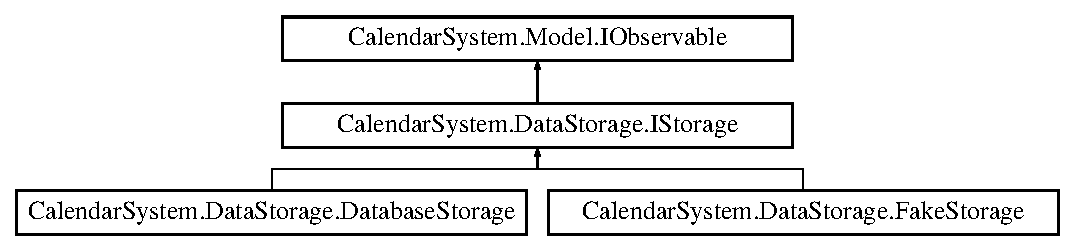
\includegraphics[height=2.926829cm]{interface_calendar_system_1_1_model_1_1_i_observable}
\end{center}
\end{figure}
\subsection*{Public Member Functions}
\begin{DoxyCompactItemize}
\item 
void \hyperlink{interface_calendar_system_1_1_model_1_1_i_observable_aee5d17758abde1cd470266ede5fab0c1}{Notify\+Observers} ()
\begin{DoxyCompactList}\small\item\em Notify observers that a change has happened. \end{DoxyCompactList}\item 
void \hyperlink{interface_calendar_system_1_1_model_1_1_i_observable_a23ca77451b9e6b19cdc111e0ef5f87c6}{Be\+Observed} (\hyperlink{interface_calendar_system_1_1_model_1_1_i_observer}{I\+Observer} observer)
\begin{DoxyCompactList}\small\item\em Become observed by an object which class has implemented \hyperlink{interface_calendar_system_1_1_model_1_1_i_observer}{I\+Observer} \end{DoxyCompactList}\item 
void \hyperlink{interface_calendar_system_1_1_model_1_1_i_observable_a53350aea0b6bf4ef1266d5d955db4700}{Be\+Observed} (I\+List$<$ \hyperlink{interface_calendar_system_1_1_model_1_1_i_observer}{I\+Observer} $>$ observers)
\begin{DoxyCompactList}\small\item\em Be observed by a list of I\+Observer(s). \end{DoxyCompactList}\end{DoxyCompactItemize}


\subsection{Detailed Description}
The interface for observable objects. Used to implement the observer pattern, such that the model can notify the view(controller) 



\subsection{Member Function Documentation}
\hypertarget{interface_calendar_system_1_1_model_1_1_i_observable_a23ca77451b9e6b19cdc111e0ef5f87c6}{\index{Calendar\+System\+::\+Model\+::\+I\+Observable@{Calendar\+System\+::\+Model\+::\+I\+Observable}!Be\+Observed@{Be\+Observed}}
\index{Be\+Observed@{Be\+Observed}!Calendar\+System\+::\+Model\+::\+I\+Observable@{Calendar\+System\+::\+Model\+::\+I\+Observable}}
\subsubsection[{Be\+Observed}]{\setlength{\rightskip}{0pt plus 5cm}void Calendar\+System.\+Model.\+I\+Observable.\+Be\+Observed (
\begin{DoxyParamCaption}
\item[{{\bf I\+Observer}}]{observer}
\end{DoxyParamCaption}
)}}\label{interface_calendar_system_1_1_model_1_1_i_observable_a23ca77451b9e6b19cdc111e0ef5f87c6}


Become observed by an object which class has implemented \hyperlink{interface_calendar_system_1_1_model_1_1_i_observer}{I\+Observer} 


\begin{DoxyParams}{Parameters}
{\em observer} & \\
\hline
\end{DoxyParams}


Implemented in \hyperlink{class_calendar_system_1_1_data_storage_1_1_database_storage_a6a80bdff8f3619508f20afdb3dddf650}{Calendar\+System.\+Data\+Storage.\+Database\+Storage}, and \hyperlink{class_calendar_system_1_1_data_storage_1_1_fake_storage_a145d71dfbca477a39bbd5c865f2e10fe}{Calendar\+System.\+Data\+Storage.\+Fake\+Storage}.

\hypertarget{interface_calendar_system_1_1_model_1_1_i_observable_a53350aea0b6bf4ef1266d5d955db4700}{\index{Calendar\+System\+::\+Model\+::\+I\+Observable@{Calendar\+System\+::\+Model\+::\+I\+Observable}!Be\+Observed@{Be\+Observed}}
\index{Be\+Observed@{Be\+Observed}!Calendar\+System\+::\+Model\+::\+I\+Observable@{Calendar\+System\+::\+Model\+::\+I\+Observable}}
\subsubsection[{Be\+Observed}]{\setlength{\rightskip}{0pt plus 5cm}void Calendar\+System.\+Model.\+I\+Observable.\+Be\+Observed (
\begin{DoxyParamCaption}
\item[{I\+List$<$ {\bf I\+Observer} $>$}]{observers}
\end{DoxyParamCaption}
)}}\label{interface_calendar_system_1_1_model_1_1_i_observable_a53350aea0b6bf4ef1266d5d955db4700}


Be observed by a list of I\+Observer(s). 


\begin{DoxyParams}{Parameters}
{\em observers} & \\
\hline
\end{DoxyParams}


Implemented in \hyperlink{class_calendar_system_1_1_data_storage_1_1_database_storage_a21c41a45e85e0ace4e49838659587934}{Calendar\+System.\+Data\+Storage.\+Database\+Storage}, and \hyperlink{class_calendar_system_1_1_data_storage_1_1_fake_storage_ab9861bbbb0b5f5af8928f4c7efec59b5}{Calendar\+System.\+Data\+Storage.\+Fake\+Storage}.

\hypertarget{interface_calendar_system_1_1_model_1_1_i_observable_aee5d17758abde1cd470266ede5fab0c1}{\index{Calendar\+System\+::\+Model\+::\+I\+Observable@{Calendar\+System\+::\+Model\+::\+I\+Observable}!Notify\+Observers@{Notify\+Observers}}
\index{Notify\+Observers@{Notify\+Observers}!Calendar\+System\+::\+Model\+::\+I\+Observable@{Calendar\+System\+::\+Model\+::\+I\+Observable}}
\subsubsection[{Notify\+Observers}]{\setlength{\rightskip}{0pt plus 5cm}void Calendar\+System.\+Model.\+I\+Observable.\+Notify\+Observers (
\begin{DoxyParamCaption}
{}
\end{DoxyParamCaption}
)}}\label{interface_calendar_system_1_1_model_1_1_i_observable_aee5d17758abde1cd470266ede5fab0c1}


Notify observers that a change has happened. 



Implemented in \hyperlink{class_calendar_system_1_1_data_storage_1_1_database_storage_a9dde52dd67fc234b5f4ed217801968af}{Calendar\+System.\+Data\+Storage.\+Database\+Storage}, and \hyperlink{class_calendar_system_1_1_data_storage_1_1_fake_storage_ad141dac914a11365efa50b8bf1bcc80d}{Calendar\+System.\+Data\+Storage.\+Fake\+Storage}.



The documentation for this interface was generated from the following file\+:\begin{DoxyCompactItemize}
\item 
Calendar\+System/\+Model/I\+Observable.\+cs\end{DoxyCompactItemize}

\hypertarget{interface_calendar_system_1_1_model_1_1_i_observer}{\section{Calendar\+System.\+Model.\+I\+Observer Interface Reference}
\label{interface_calendar_system_1_1_model_1_1_i_observer}\index{Calendar\+System.\+Model.\+I\+Observer@{Calendar\+System.\+Model.\+I\+Observer}}
}


The interface for observing objects. Used to implement the observer pattern, such that the model can notify the view(controller)  


Inheritance diagram for Calendar\+System.\+Model.\+I\+Observer\+:\begin{figure}[H]
\begin{center}
\leavevmode
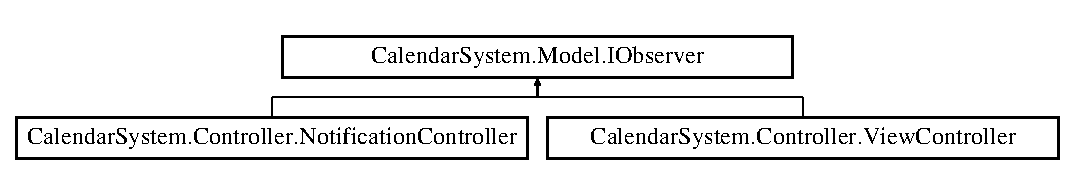
\includegraphics[height=1.898305cm]{interface_calendar_system_1_1_model_1_1_i_observer}
\end{center}
\end{figure}
\subsection*{Public Member Functions}
\begin{DoxyCompactItemize}
\item 
void \hyperlink{interface_calendar_system_1_1_model_1_1_i_observer_a87a0dd14cdbb1ae4b4531329011167fb}{Be\+Notified\+By\+Observed} ()
\begin{DoxyCompactList}\small\item\em A method which is called from the \hyperlink{interface_calendar_system_1_1_model_1_1_i_observable}{I\+Observable} objects which the \hyperlink{interface_calendar_system_1_1_model_1_1_i_observer}{I\+Observer} has observed. The method notifies that the \hyperlink{interface_calendar_system_1_1_model_1_1_i_observable}{I\+Observable} has been updated. \end{DoxyCompactList}\end{DoxyCompactItemize}


\subsection{Detailed Description}
The interface for observing objects. Used to implement the observer pattern, such that the model can notify the view(controller) 



\subsection{Member Function Documentation}
\hypertarget{interface_calendar_system_1_1_model_1_1_i_observer_a87a0dd14cdbb1ae4b4531329011167fb}{\index{Calendar\+System\+::\+Model\+::\+I\+Observer@{Calendar\+System\+::\+Model\+::\+I\+Observer}!Be\+Notified\+By\+Observed@{Be\+Notified\+By\+Observed}}
\index{Be\+Notified\+By\+Observed@{Be\+Notified\+By\+Observed}!Calendar\+System\+::\+Model\+::\+I\+Observer@{Calendar\+System\+::\+Model\+::\+I\+Observer}}
\subsubsection[{Be\+Notified\+By\+Observed}]{\setlength{\rightskip}{0pt plus 5cm}void Calendar\+System.\+Model.\+I\+Observer.\+Be\+Notified\+By\+Observed (
\begin{DoxyParamCaption}
{}
\end{DoxyParamCaption}
)}}\label{interface_calendar_system_1_1_model_1_1_i_observer_a87a0dd14cdbb1ae4b4531329011167fb}


A method which is called from the \hyperlink{interface_calendar_system_1_1_model_1_1_i_observable}{I\+Observable} objects which the \hyperlink{interface_calendar_system_1_1_model_1_1_i_observer}{I\+Observer} has observed. The method notifies that the \hyperlink{interface_calendar_system_1_1_model_1_1_i_observable}{I\+Observable} has been updated. 



Implemented in \hyperlink{class_calendar_system_1_1_controller_1_1_view_controller_a46f9d0983af0da3f95e00e4047d685a5}{Calendar\+System.\+Controller.\+View\+Controller}, and \hyperlink{class_calendar_system_1_1_controller_1_1_notification_controller_a1f57126c0b90cb4b4ab54b599d83035c}{Calendar\+System.\+Controller.\+Notification\+Controller}.



The documentation for this interface was generated from the following file\+:\begin{DoxyCompactItemize}
\item 
Calendar\+System/\+Model/I\+Observer.\+cs\end{DoxyCompactItemize}

\hypertarget{interface_calendar_system_1_1_data_storage_1_1_i_storage}{\section{Calendar\+System.\+Data\+Storage.\+I\+Storage Interface Reference}
\label{interface_calendar_system_1_1_data_storage_1_1_i_storage}\index{Calendar\+System.\+Data\+Storage.\+I\+Storage@{Calendar\+System.\+Data\+Storage.\+I\+Storage}}
}


An interface for a storage class. The interface has methods which will make it possible to get and save events into the calendar, without knowing the actual implementation.  


Inheritance diagram for Calendar\+System.\+Data\+Storage.\+I\+Storage\+:\begin{figure}[H]
\begin{center}
\leavevmode
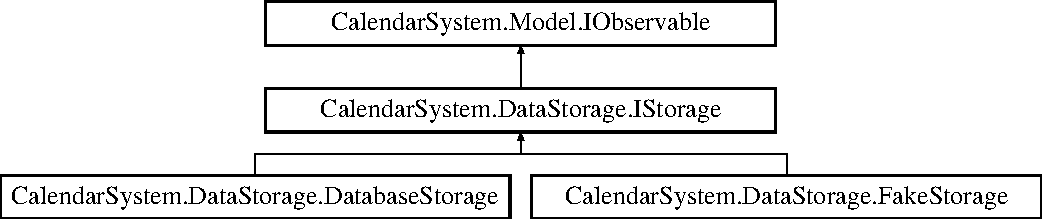
\includegraphics[height=2.926829cm]{interface_calendar_system_1_1_data_storage_1_1_i_storage}
\end{center}
\end{figure}
\subsection*{Public Member Functions}
\begin{DoxyCompactItemize}
\item 
void \hyperlink{interface_calendar_system_1_1_data_storage_1_1_i_storage_a7818cf23c7f6dfca608c175d70558aa6}{login\+Authentication} (string user\+Name, string password)
\begin{DoxyCompactList}\small\item\em Authenticate and download Calendar and events belonging to that user. \end{DoxyCompactList}\item 
void \hyperlink{interface_calendar_system_1_1_data_storage_1_1_i_storage_a041366475064bd7008e0546ac8d5d148}{Save\+Event} (string description, Date\+Time date\+Time, Time\+Span time\+Span, \hyperlink{class_calendar_system_1_1_model_1_1_notification}{Notification} notification)
\begin{DoxyCompactList}\small\item\em Save an event to the storage \end{DoxyCompactList}\item 
void \hyperlink{interface_calendar_system_1_1_data_storage_1_1_i_storage_a671ad7560e3d8197ec7867e98d3c138e}{Update\+Event} (int I\+D, string description, Date\+Time date\+Time, Time\+Span time\+Span, \hyperlink{class_calendar_system_1_1_model_1_1_notification}{Notification} notification)
\begin{DoxyCompactList}\small\item\em Update an event to the storage \end{DoxyCompactList}\item 
I\+List$<$ \hyperlink{interface_calendar_system_1_1_model_1_1_i_event}{I\+Event} $>$ \hyperlink{interface_calendar_system_1_1_data_storage_1_1_i_storage_a06b5b139e4ef5fc7e66be8ffad9aed82}{Get\+All\+Events} ()
\begin{DoxyCompactList}\small\item\em Returns all events in the active calendar \end{DoxyCompactList}\item 
\hyperlink{interface_calendar_system_1_1_model_1_1_i_event}{I\+Event} \hyperlink{interface_calendar_system_1_1_data_storage_1_1_i_storage_a9b144e859410dbe90cc0876750c2872f}{Get\+Event} (int I\+D)
\begin{DoxyCompactList}\small\item\em Get a single event with a given I\+D if possible. \end{DoxyCompactList}\item 
I\+List$<$ \hyperlink{interface_calendar_system_1_1_model_1_1_i_event}{I\+Event} $>$ \hyperlink{interface_calendar_system_1_1_data_storage_1_1_i_storage_a1547353aae64841c1a79d60f07384c99}{Get\+Events\+Between\+Dates} (Date\+Time begin\+Date\+Time, Date\+Time en\+Date\+Time)
\begin{DoxyCompactList}\small\item\em Return all events between to given dates. \end{DoxyCompactList}\item 
void \hyperlink{interface_calendar_system_1_1_data_storage_1_1_i_storage_a8831822c54d654f17c98a8b13e679240}{Create\+Tag} (\hyperlink{class_calendar_system_1_1_model_1_1_tag}{Tag} tag)
\begin{DoxyCompactList}\small\item\em Create a tag and save it in the storage. \end{DoxyCompactList}\end{DoxyCompactItemize}


\subsection{Detailed Description}
An interface for a storage class. The interface has methods which will make it possible to get and save events into the calendar, without knowing the actual implementation. 



\subsection{Member Function Documentation}
\hypertarget{interface_calendar_system_1_1_data_storage_1_1_i_storage_a8831822c54d654f17c98a8b13e679240}{\index{Calendar\+System\+::\+Data\+Storage\+::\+I\+Storage@{Calendar\+System\+::\+Data\+Storage\+::\+I\+Storage}!Create\+Tag@{Create\+Tag}}
\index{Create\+Tag@{Create\+Tag}!Calendar\+System\+::\+Data\+Storage\+::\+I\+Storage@{Calendar\+System\+::\+Data\+Storage\+::\+I\+Storage}}
\subsubsection[{Create\+Tag}]{\setlength{\rightskip}{0pt plus 5cm}void Calendar\+System.\+Data\+Storage.\+I\+Storage.\+Create\+Tag (
\begin{DoxyParamCaption}
\item[{{\bf Tag}}]{tag}
\end{DoxyParamCaption}
)}}\label{interface_calendar_system_1_1_data_storage_1_1_i_storage_a8831822c54d654f17c98a8b13e679240}


Create a tag and save it in the storage. 


\begin{DoxyParams}{Parameters}
{\em tag} & \\
\hline
\end{DoxyParams}


Implemented in \hyperlink{class_calendar_system_1_1_data_storage_1_1_database_storage_aee69c1fc20000371ee89ac06617d3610}{Calendar\+System.\+Data\+Storage.\+Database\+Storage}, and \hyperlink{class_calendar_system_1_1_data_storage_1_1_fake_storage_a713df02585d277ddb922d5912ad4a592}{Calendar\+System.\+Data\+Storage.\+Fake\+Storage}.

\hypertarget{interface_calendar_system_1_1_data_storage_1_1_i_storage_a06b5b139e4ef5fc7e66be8ffad9aed82}{\index{Calendar\+System\+::\+Data\+Storage\+::\+I\+Storage@{Calendar\+System\+::\+Data\+Storage\+::\+I\+Storage}!Get\+All\+Events@{Get\+All\+Events}}
\index{Get\+All\+Events@{Get\+All\+Events}!Calendar\+System\+::\+Data\+Storage\+::\+I\+Storage@{Calendar\+System\+::\+Data\+Storage\+::\+I\+Storage}}
\subsubsection[{Get\+All\+Events}]{\setlength{\rightskip}{0pt plus 5cm}I\+List$<${\bf I\+Event}$>$ Calendar\+System.\+Data\+Storage.\+I\+Storage.\+Get\+All\+Events (
\begin{DoxyParamCaption}
{}
\end{DoxyParamCaption}
)}}\label{interface_calendar_system_1_1_data_storage_1_1_i_storage_a06b5b139e4ef5fc7e66be8ffad9aed82}


Returns all events in the active calendar 

\begin{DoxyReturn}{Returns}

\end{DoxyReturn}


Implemented in \hyperlink{class_calendar_system_1_1_data_storage_1_1_database_storage_ab28e18e900a2011f271239952d9e2e26}{Calendar\+System.\+Data\+Storage.\+Database\+Storage}, and \hyperlink{class_calendar_system_1_1_data_storage_1_1_fake_storage_a2b5d3fab2d4db84aa279e1408f56abb2}{Calendar\+System.\+Data\+Storage.\+Fake\+Storage}.

\hypertarget{interface_calendar_system_1_1_data_storage_1_1_i_storage_a9b144e859410dbe90cc0876750c2872f}{\index{Calendar\+System\+::\+Data\+Storage\+::\+I\+Storage@{Calendar\+System\+::\+Data\+Storage\+::\+I\+Storage}!Get\+Event@{Get\+Event}}
\index{Get\+Event@{Get\+Event}!Calendar\+System\+::\+Data\+Storage\+::\+I\+Storage@{Calendar\+System\+::\+Data\+Storage\+::\+I\+Storage}}
\subsubsection[{Get\+Event}]{\setlength{\rightskip}{0pt plus 5cm}{\bf I\+Event} Calendar\+System.\+Data\+Storage.\+I\+Storage.\+Get\+Event (
\begin{DoxyParamCaption}
\item[{int}]{I\+D}
\end{DoxyParamCaption}
)}}\label{interface_calendar_system_1_1_data_storage_1_1_i_storage_a9b144e859410dbe90cc0876750c2872f}


Get a single event with a given I\+D if possible. 


\begin{DoxyParams}{Parameters}
{\em I\+D} & \\
\hline
\end{DoxyParams}
\begin{DoxyReturn}{Returns}

\end{DoxyReturn}


Implemented in \hyperlink{class_calendar_system_1_1_data_storage_1_1_database_storage_a792702533aed5e26a856b216dffb67b4}{Calendar\+System.\+Data\+Storage.\+Database\+Storage}, and \hyperlink{class_calendar_system_1_1_data_storage_1_1_fake_storage_a6f614104bbd16f6f04179dc6e7b41dd1}{Calendar\+System.\+Data\+Storage.\+Fake\+Storage}.

\hypertarget{interface_calendar_system_1_1_data_storage_1_1_i_storage_a1547353aae64841c1a79d60f07384c99}{\index{Calendar\+System\+::\+Data\+Storage\+::\+I\+Storage@{Calendar\+System\+::\+Data\+Storage\+::\+I\+Storage}!Get\+Events\+Between\+Dates@{Get\+Events\+Between\+Dates}}
\index{Get\+Events\+Between\+Dates@{Get\+Events\+Between\+Dates}!Calendar\+System\+::\+Data\+Storage\+::\+I\+Storage@{Calendar\+System\+::\+Data\+Storage\+::\+I\+Storage}}
\subsubsection[{Get\+Events\+Between\+Dates}]{\setlength{\rightskip}{0pt plus 5cm}I\+List$<${\bf I\+Event}$>$ Calendar\+System.\+Data\+Storage.\+I\+Storage.\+Get\+Events\+Between\+Dates (
\begin{DoxyParamCaption}
\item[{Date\+Time}]{begin\+Date\+Time, }
\item[{Date\+Time}]{en\+Date\+Time}
\end{DoxyParamCaption}
)}}\label{interface_calendar_system_1_1_data_storage_1_1_i_storage_a1547353aae64841c1a79d60f07384c99}


Return all events between to given dates. 


\begin{DoxyParams}{Parameters}
{\em begin\+Date\+Time} & \\
\hline
{\em en\+Date\+Time} & \\
\hline
\end{DoxyParams}
\begin{DoxyReturn}{Returns}

\end{DoxyReturn}


Implemented in \hyperlink{class_calendar_system_1_1_data_storage_1_1_database_storage_a168ecf83f6b5d8686fedd72c422b4486}{Calendar\+System.\+Data\+Storage.\+Database\+Storage}, and \hyperlink{class_calendar_system_1_1_data_storage_1_1_fake_storage_a16ce769932055ee3cc1bd47e945e7cfe}{Calendar\+System.\+Data\+Storage.\+Fake\+Storage}.

\hypertarget{interface_calendar_system_1_1_data_storage_1_1_i_storage_a7818cf23c7f6dfca608c175d70558aa6}{\index{Calendar\+System\+::\+Data\+Storage\+::\+I\+Storage@{Calendar\+System\+::\+Data\+Storage\+::\+I\+Storage}!login\+Authentication@{login\+Authentication}}
\index{login\+Authentication@{login\+Authentication}!Calendar\+System\+::\+Data\+Storage\+::\+I\+Storage@{Calendar\+System\+::\+Data\+Storage\+::\+I\+Storage}}
\subsubsection[{login\+Authentication}]{\setlength{\rightskip}{0pt plus 5cm}void Calendar\+System.\+Data\+Storage.\+I\+Storage.\+login\+Authentication (
\begin{DoxyParamCaption}
\item[{string}]{user\+Name, }
\item[{string}]{password}
\end{DoxyParamCaption}
)}}\label{interface_calendar_system_1_1_data_storage_1_1_i_storage_a7818cf23c7f6dfca608c175d70558aa6}


Authenticate and download Calendar and events belonging to that user. 


\begin{DoxyParams}{Parameters}
{\em user\+Name} & \\
\hline
{\em password} & \\
\hline
\end{DoxyParams}
\begin{DoxyReturn}{Returns}

\end{DoxyReturn}


Implemented in \hyperlink{class_calendar_system_1_1_data_storage_1_1_database_storage_a3c7ccd413ae0f0d4684cf1b1998cddcd}{Calendar\+System.\+Data\+Storage.\+Database\+Storage}, and \hyperlink{class_calendar_system_1_1_data_storage_1_1_fake_storage_a589c203e56e50f0e71a1d202f7411a2f}{Calendar\+System.\+Data\+Storage.\+Fake\+Storage}.

\hypertarget{interface_calendar_system_1_1_data_storage_1_1_i_storage_a041366475064bd7008e0546ac8d5d148}{\index{Calendar\+System\+::\+Data\+Storage\+::\+I\+Storage@{Calendar\+System\+::\+Data\+Storage\+::\+I\+Storage}!Save\+Event@{Save\+Event}}
\index{Save\+Event@{Save\+Event}!Calendar\+System\+::\+Data\+Storage\+::\+I\+Storage@{Calendar\+System\+::\+Data\+Storage\+::\+I\+Storage}}
\subsubsection[{Save\+Event}]{\setlength{\rightskip}{0pt plus 5cm}void Calendar\+System.\+Data\+Storage.\+I\+Storage.\+Save\+Event (
\begin{DoxyParamCaption}
\item[{string}]{description, }
\item[{Date\+Time}]{date\+Time, }
\item[{Time\+Span}]{time\+Span, }
\item[{{\bf Notification}}]{notification}
\end{DoxyParamCaption}
)}}\label{interface_calendar_system_1_1_data_storage_1_1_i_storage_a041366475064bd7008e0546ac8d5d148}


Save an event to the storage 


\begin{DoxyParams}{Parameters}
{\em description} & \\
\hline
{\em date\+Time} & \\
\hline
{\em time\+Span} & \\
\hline
{\em notification} & \\
\hline
\end{DoxyParams}


Implemented in \hyperlink{class_calendar_system_1_1_data_storage_1_1_database_storage_ae4e6526f9d99e4a01b75a591a15fba9c}{Calendar\+System.\+Data\+Storage.\+Database\+Storage}, and \hyperlink{class_calendar_system_1_1_data_storage_1_1_fake_storage_ac59fb43db4eb01c5b6153c7919608313}{Calendar\+System.\+Data\+Storage.\+Fake\+Storage}.

\hypertarget{interface_calendar_system_1_1_data_storage_1_1_i_storage_a671ad7560e3d8197ec7867e98d3c138e}{\index{Calendar\+System\+::\+Data\+Storage\+::\+I\+Storage@{Calendar\+System\+::\+Data\+Storage\+::\+I\+Storage}!Update\+Event@{Update\+Event}}
\index{Update\+Event@{Update\+Event}!Calendar\+System\+::\+Data\+Storage\+::\+I\+Storage@{Calendar\+System\+::\+Data\+Storage\+::\+I\+Storage}}
\subsubsection[{Update\+Event}]{\setlength{\rightskip}{0pt plus 5cm}void Calendar\+System.\+Data\+Storage.\+I\+Storage.\+Update\+Event (
\begin{DoxyParamCaption}
\item[{int}]{I\+D, }
\item[{string}]{description, }
\item[{Date\+Time}]{date\+Time, }
\item[{Time\+Span}]{time\+Span, }
\item[{{\bf Notification}}]{notification}
\end{DoxyParamCaption}
)}}\label{interface_calendar_system_1_1_data_storage_1_1_i_storage_a671ad7560e3d8197ec7867e98d3c138e}


Update an event to the storage 


\begin{DoxyParams}{Parameters}
{\em description} & \\
\hline
{\em date\+Time} & \\
\hline
{\em time\+Span} & \\
\hline
{\em notification} & \\
\hline
\end{DoxyParams}


Implemented in \hyperlink{class_calendar_system_1_1_data_storage_1_1_database_storage_a9be31393f6b29a9b1b09297153da6b87}{Calendar\+System.\+Data\+Storage.\+Database\+Storage}, and \hyperlink{class_calendar_system_1_1_data_storage_1_1_fake_storage_a0d2bffbcf0485788321dbde8b419fc13}{Calendar\+System.\+Data\+Storage.\+Fake\+Storage}.



The documentation for this interface was generated from the following file\+:\begin{DoxyCompactItemize}
\item 
Calendar\+System/\+Data\+Storage/I\+Storage.\+cs\end{DoxyCompactItemize}

\hypertarget{class_calendar_system_1_1_view_1_1_login_view}{\section{Calendar\+System.\+View.\+Login\+View Class Reference}
\label{class_calendar_system_1_1_view_1_1_login_view}\index{Calendar\+System.\+View.\+Login\+View@{Calendar\+System.\+View.\+Login\+View}}
}


The login view is the view which is prompted to the user first. It contains two textboxes and a login button.  




\subsection{Detailed Description}
The login view is the view which is prompted to the user first. It contains two textboxes and a login button. 



The documentation for this class was generated from the following file\+:\begin{DoxyCompactItemize}
\item 
Calendar\+System/\+View/Login\+View.\+cs\end{DoxyCompactItemize}

\hypertarget{class_calendar_system_1_1_view_1_1_main_view}{\section{Calendar\+System.\+View.\+Main\+View Class Reference}
\label{class_calendar_system_1_1_view_1_1_main_view}\index{Calendar\+System.\+View.\+Main\+View@{Calendar\+System.\+View.\+Main\+View}}
}


The main view is the container of the other views as well as search bars, properties and so on.  


\subsection*{Public Member Functions}
\begin{DoxyCompactItemize}
\item 
\hypertarget{class_calendar_system_1_1_view_1_1_main_view_aed8181268948a63772e2b864f0191849}{{\bfseries Main\+View} (\hyperlink{class_calendar_system_1_1_view_1_1_calendar_view}{Calendar\+View} calendar\+View)}\label{class_calendar_system_1_1_view_1_1_main_view_aed8181268948a63772e2b864f0191849}

\end{DoxyCompactItemize}


\subsection{Detailed Description}
The main view is the container of the other views as well as search bars, properties and so on. 



The documentation for this class was generated from the following file\+:\begin{DoxyCompactItemize}
\item 
Calendar\+System/\+View/Main\+View.\+cs\end{DoxyCompactItemize}

\hypertarget{class_calendar_system_1_1_model_1_1_notification}{\section{Calendar\+System.\+Model.\+Notification Class Reference}
\label{class_calendar_system_1_1_model_1_1_notification}\index{Calendar\+System.\+Model.\+Notification@{Calendar\+System.\+Model.\+Notification}}
}


A class which has a date for when the notification enters an alarmstate and a description.  


\subsection*{Public Member Functions}
\begin{DoxyCompactItemize}
\item 
\hypertarget{class_calendar_system_1_1_model_1_1_notification_a802f3c38e95194ced78a5b707ac26899}{{\bfseries Notification} (Date\+Time date, string description)}\label{class_calendar_system_1_1_model_1_1_notification_a802f3c38e95194ced78a5b707ac26899}

\item 
\hypertarget{class_calendar_system_1_1_model_1_1_notification_ab3ebc86292f1f4382f85c72fce000125}{bool {\bfseries is\+In\+Alarm\+State} ()}\label{class_calendar_system_1_1_model_1_1_notification_ab3ebc86292f1f4382f85c72fce000125}

\end{DoxyCompactItemize}


\subsection{Detailed Description}
A class which has a date for when the notification enters an alarmstate and a description. 



The documentation for this class was generated from the following file\+:\begin{DoxyCompactItemize}
\item 
Calendar\+System/\+Model/Notification.\+cs\end{DoxyCompactItemize}

\hypertarget{class_calendar_system_1_1_controller_1_1_notification_controller}{\section{Calendar\+System.\+Controller.\+Notification\+Controller Class Reference}
\label{class_calendar_system_1_1_controller_1_1_notification_controller}\index{Calendar\+System.\+Controller.\+Notification\+Controller@{Calendar\+System.\+Controller.\+Notification\+Controller}}
}


The Notification controller has a timer for the notifications and will create a popup when a notification's time is exceeded.  


Inheritance diagram for Calendar\+System.\+Controller.\+Notification\+Controller\+:\begin{figure}[H]
\begin{center}
\leavevmode
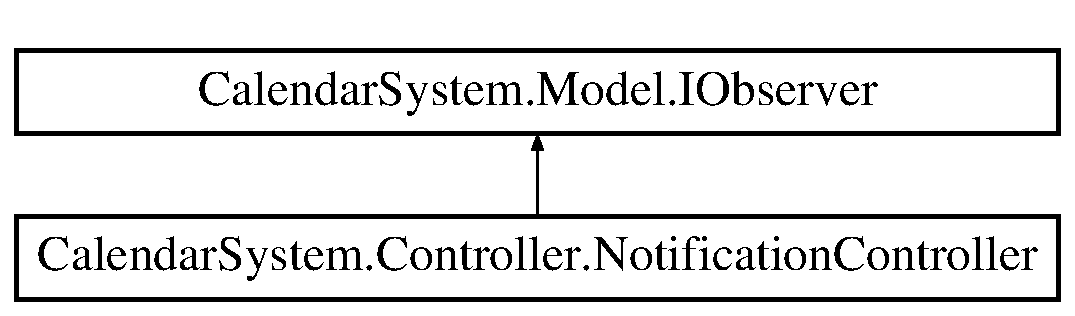
\includegraphics[height=2.000000cm]{class_calendar_system_1_1_controller_1_1_notification_controller}
\end{center}
\end{figure}
\subsection*{Public Member Functions}
\begin{DoxyCompactItemize}
\item 
void \hyperlink{class_calendar_system_1_1_controller_1_1_notification_controller_a1f57126c0b90cb4b4ab54b599d83035c}{Be\+Notified\+By\+Observed} ()
\begin{DoxyCompactList}\small\item\em A change in the model has happened. \end{DoxyCompactList}\end{DoxyCompactItemize}
\subsection*{Static Public Member Functions}
\begin{DoxyCompactItemize}
\item 
static \hyperlink{class_calendar_system_1_1_controller_1_1_notification_controller}{Notification\+Controller} \hyperlink{class_calendar_system_1_1_controller_1_1_notification_controller_aee114fb47d6d78ae8794f2504584e946}{get\+Instance} ()
\begin{DoxyCompactList}\small\item\em Singleton pattern. Makes sure only one instance can exist at a given time, and give classes easy access to the controller. \end{DoxyCompactList}\end{DoxyCompactItemize}


\subsection{Detailed Description}
The Notification controller has a timer for the notifications and will create a popup when a notification's time is exceeded. 



\subsection{Member Function Documentation}
\hypertarget{class_calendar_system_1_1_controller_1_1_notification_controller_a1f57126c0b90cb4b4ab54b599d83035c}{\index{Calendar\+System\+::\+Controller\+::\+Notification\+Controller@{Calendar\+System\+::\+Controller\+::\+Notification\+Controller}!Be\+Notified\+By\+Observed@{Be\+Notified\+By\+Observed}}
\index{Be\+Notified\+By\+Observed@{Be\+Notified\+By\+Observed}!Calendar\+System\+::\+Controller\+::\+Notification\+Controller@{Calendar\+System\+::\+Controller\+::\+Notification\+Controller}}
\subsubsection[{Be\+Notified\+By\+Observed}]{\setlength{\rightskip}{0pt plus 5cm}void Calendar\+System.\+Controller.\+Notification\+Controller.\+Be\+Notified\+By\+Observed (
\begin{DoxyParamCaption}
{}
\end{DoxyParamCaption}
)}}\label{class_calendar_system_1_1_controller_1_1_notification_controller_a1f57126c0b90cb4b4ab54b599d83035c}


A change in the model has happened. 



Implements \hyperlink{interface_calendar_system_1_1_model_1_1_i_observer_a87a0dd14cdbb1ae4b4531329011167fb}{Calendar\+System.\+Model.\+I\+Observer}.

\hypertarget{class_calendar_system_1_1_controller_1_1_notification_controller_aee114fb47d6d78ae8794f2504584e946}{\index{Calendar\+System\+::\+Controller\+::\+Notification\+Controller@{Calendar\+System\+::\+Controller\+::\+Notification\+Controller}!get\+Instance@{get\+Instance}}
\index{get\+Instance@{get\+Instance}!Calendar\+System\+::\+Controller\+::\+Notification\+Controller@{Calendar\+System\+::\+Controller\+::\+Notification\+Controller}}
\subsubsection[{get\+Instance}]{\setlength{\rightskip}{0pt plus 5cm}static {\bf Notification\+Controller} Calendar\+System.\+Controller.\+Notification\+Controller.\+get\+Instance (
\begin{DoxyParamCaption}
{}
\end{DoxyParamCaption}
)\hspace{0.3cm}{\ttfamily [static]}}}\label{class_calendar_system_1_1_controller_1_1_notification_controller_aee114fb47d6d78ae8794f2504584e946}


Singleton pattern. Makes sure only one instance can exist at a given time, and give classes easy access to the controller. 

\begin{DoxyReturn}{Returns}
The only instance of the class
\end{DoxyReturn}


The documentation for this class was generated from the following file\+:\begin{DoxyCompactItemize}
\item 
Calendar\+System/\+Controller/Notification\+Controller.\+cs\end{DoxyCompactItemize}

\hypertarget{class_calendar_system_1_1_view_1_1_notification_view}{\section{Calendar\+System.\+View.\+Notification\+View Class Reference}
\label{class_calendar_system_1_1_view_1_1_notification_view}\index{Calendar\+System.\+View.\+Notification\+View@{Calendar\+System.\+View.\+Notification\+View}}
}


A class that visually represents an notification object, or the creation thereof.  




\subsection{Detailed Description}
A class that visually represents an notification object, or the creation thereof. 



The documentation for this class was generated from the following file\+:\begin{DoxyCompactItemize}
\item 
Calendar\+System/\+View/Notification\+View.\+cs\end{DoxyCompactItemize}

\hypertarget{class_calendar_system_1_1_model_1_1_tag}{\section{Calendar\+System.\+Model.\+Tag Class Reference}
\label{class_calendar_system_1_1_model_1_1_tag}\index{Calendar\+System.\+Model.\+Tag@{Calendar\+System.\+Model.\+Tag}}
}


Implementation is unclear for now  


\subsection*{Public Member Functions}
\begin{DoxyCompactItemize}
\item 
\hypertarget{class_calendar_system_1_1_model_1_1_tag_ada523979bd87a2161b41acad504e2a4f}{void {\bfseries create\+Tags} (string new\+Tag, Color new\+Color)}\label{class_calendar_system_1_1_model_1_1_tag_ada523979bd87a2161b41acad504e2a4f}

\end{DoxyCompactItemize}


\subsection{Detailed Description}
Implementation is unclear for now 



The documentation for this class was generated from the following file\+:\begin{DoxyCompactItemize}
\item 
Calendar\+System/\+Model/Tag.\+cs\end{DoxyCompactItemize}

\hypertarget{class_calendar_system_1_1_controller_1_1_view_controller}{\section{Calendar\+System.\+Controller.\+View\+Controller Class Reference}
\label{class_calendar_system_1_1_controller_1_1_view_controller}\index{Calendar\+System.\+Controller.\+View\+Controller@{Calendar\+System.\+Controller.\+View\+Controller}}
}


The view controller handles all calls and creations of the view. It implements the I\+Observer interface and therefore can get notified when changes in the model happens.  


Inheritance diagram for Calendar\+System.\+Controller.\+View\+Controller\+:\begin{figure}[H]
\begin{center}
\leavevmode
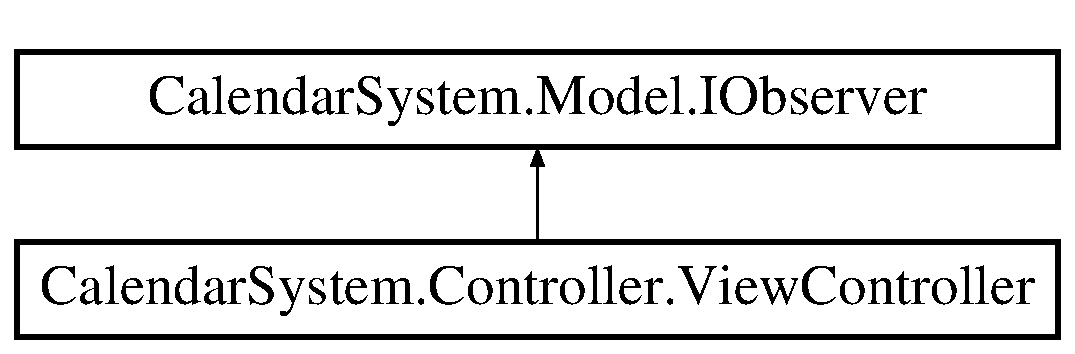
\includegraphics[height=2.000000cm]{class_calendar_system_1_1_controller_1_1_view_controller}
\end{center}
\end{figure}
\subsection*{Public Member Functions}
\begin{DoxyCompactItemize}
\item 
void \hyperlink{class_calendar_system_1_1_controller_1_1_view_controller_a70e4c5e8dd89b0dbd3f8da0d39ab652b}{start\+Main\+View} ()
\begin{DoxyCompactList}\small\item\em Create the main view \end{DoxyCompactList}\item 
void \hyperlink{class_calendar_system_1_1_controller_1_1_view_controller_a6f51cc970fd23a5cfa9c861af874be9e}{create\+Event\+View} ()
\begin{DoxyCompactList}\small\item\em Create a new event view \end{DoxyCompactList}\item 
\hypertarget{class_calendar_system_1_1_controller_1_1_view_controller_a5ccc036864876db5c50e549ba2ab8093}{void {\bfseries create\+Notification\+View} (int I\+D, \hyperlink{class_calendar_system_1_1_model_1_1_notification}{Notification} notification)}\label{class_calendar_system_1_1_controller_1_1_view_controller_a5ccc036864876db5c50e549ba2ab8093}

\item 
void \hyperlink{class_calendar_system_1_1_controller_1_1_view_controller_a536858a1ed8b64b91a0b06d42c62875a}{create\+Event\+View} (\hyperlink{interface_calendar_system_1_1_model_1_1_i_event}{I\+Event} i\+Event)
\begin{DoxyCompactList}\small\item\em Create an Event view with the data from a already existing event (update event) \end{DoxyCompactList}\item 
void \hyperlink{class_calendar_system_1_1_controller_1_1_view_controller_a595641816a2e31edac5fe38f4d1f9f17}{Update\+Calender\+Overview} (string overview\+Type)
\begin{DoxyCompactList}\small\item\em Change the overviewtype of the calendarview. Right now it does not use the enum type correctly. Must be updated to properly use the enum type. \end{DoxyCompactList}\item 
void \hyperlink{class_calendar_system_1_1_controller_1_1_view_controller_a46f9d0983af0da3f95e00e4047d685a5}{Be\+Notified\+By\+Observed} ()
\begin{DoxyCompactList}\small\item\em The observable pattern method of the observers. When a change in the model has happened (the model is the observable) it has to update the calendar view. \end{DoxyCompactList}\end{DoxyCompactItemize}
\subsection*{Static Public Member Functions}
\begin{DoxyCompactItemize}
\item 
static \hyperlink{class_calendar_system_1_1_controller_1_1_view_controller}{View\+Controller} \hyperlink{class_calendar_system_1_1_controller_1_1_view_controller_ad07bc062091a439c61ba0b74f487e82d}{get\+Instance} ()
\begin{DoxyCompactList}\small\item\em Singleton pattern. Makes sure only one instance can exist at a given time, and give classes easy access to the controller. \end{DoxyCompactList}\end{DoxyCompactItemize}


\subsection{Detailed Description}
The view controller handles all calls and creations of the view. It implements the I\+Observer interface and therefore can get notified when changes in the model happens. 



\subsection{Member Function Documentation}
\hypertarget{class_calendar_system_1_1_controller_1_1_view_controller_a46f9d0983af0da3f95e00e4047d685a5}{\index{Calendar\+System\+::\+Controller\+::\+View\+Controller@{Calendar\+System\+::\+Controller\+::\+View\+Controller}!Be\+Notified\+By\+Observed@{Be\+Notified\+By\+Observed}}
\index{Be\+Notified\+By\+Observed@{Be\+Notified\+By\+Observed}!Calendar\+System\+::\+Controller\+::\+View\+Controller@{Calendar\+System\+::\+Controller\+::\+View\+Controller}}
\subsubsection[{Be\+Notified\+By\+Observed}]{\setlength{\rightskip}{0pt plus 5cm}void Calendar\+System.\+Controller.\+View\+Controller.\+Be\+Notified\+By\+Observed (
\begin{DoxyParamCaption}
{}
\end{DoxyParamCaption}
)}}\label{class_calendar_system_1_1_controller_1_1_view_controller_a46f9d0983af0da3f95e00e4047d685a5}


The observable pattern method of the observers. When a change in the model has happened (the model is the observable) it has to update the calendar view. 



Implements \hyperlink{interface_calendar_system_1_1_model_1_1_i_observer_a87a0dd14cdbb1ae4b4531329011167fb}{Calendar\+System.\+Model.\+I\+Observer}.

\hypertarget{class_calendar_system_1_1_controller_1_1_view_controller_a6f51cc970fd23a5cfa9c861af874be9e}{\index{Calendar\+System\+::\+Controller\+::\+View\+Controller@{Calendar\+System\+::\+Controller\+::\+View\+Controller}!create\+Event\+View@{create\+Event\+View}}
\index{create\+Event\+View@{create\+Event\+View}!Calendar\+System\+::\+Controller\+::\+View\+Controller@{Calendar\+System\+::\+Controller\+::\+View\+Controller}}
\subsubsection[{create\+Event\+View}]{\setlength{\rightskip}{0pt plus 5cm}void Calendar\+System.\+Controller.\+View\+Controller.\+create\+Event\+View (
\begin{DoxyParamCaption}
{}
\end{DoxyParamCaption}
)}}\label{class_calendar_system_1_1_controller_1_1_view_controller_a6f51cc970fd23a5cfa9c861af874be9e}


Create a new event view 

\hypertarget{class_calendar_system_1_1_controller_1_1_view_controller_a536858a1ed8b64b91a0b06d42c62875a}{\index{Calendar\+System\+::\+Controller\+::\+View\+Controller@{Calendar\+System\+::\+Controller\+::\+View\+Controller}!create\+Event\+View@{create\+Event\+View}}
\index{create\+Event\+View@{create\+Event\+View}!Calendar\+System\+::\+Controller\+::\+View\+Controller@{Calendar\+System\+::\+Controller\+::\+View\+Controller}}
\subsubsection[{create\+Event\+View}]{\setlength{\rightskip}{0pt plus 5cm}void Calendar\+System.\+Controller.\+View\+Controller.\+create\+Event\+View (
\begin{DoxyParamCaption}
\item[{{\bf I\+Event}}]{i\+Event}
\end{DoxyParamCaption}
)}}\label{class_calendar_system_1_1_controller_1_1_view_controller_a536858a1ed8b64b91a0b06d42c62875a}


Create an Event view with the data from a already existing event (update event) 


\begin{DoxyParams}{Parameters}
{\em i\+Event} & \\
\hline
\end{DoxyParams}
\hypertarget{class_calendar_system_1_1_controller_1_1_view_controller_ad07bc062091a439c61ba0b74f487e82d}{\index{Calendar\+System\+::\+Controller\+::\+View\+Controller@{Calendar\+System\+::\+Controller\+::\+View\+Controller}!get\+Instance@{get\+Instance}}
\index{get\+Instance@{get\+Instance}!Calendar\+System\+::\+Controller\+::\+View\+Controller@{Calendar\+System\+::\+Controller\+::\+View\+Controller}}
\subsubsection[{get\+Instance}]{\setlength{\rightskip}{0pt plus 5cm}static {\bf View\+Controller} Calendar\+System.\+Controller.\+View\+Controller.\+get\+Instance (
\begin{DoxyParamCaption}
{}
\end{DoxyParamCaption}
)\hspace{0.3cm}{\ttfamily [static]}}}\label{class_calendar_system_1_1_controller_1_1_view_controller_ad07bc062091a439c61ba0b74f487e82d}


Singleton pattern. Makes sure only one instance can exist at a given time, and give classes easy access to the controller. 

\begin{DoxyReturn}{Returns}
The only instance of the class
\end{DoxyReturn}
\hypertarget{class_calendar_system_1_1_controller_1_1_view_controller_a70e4c5e8dd89b0dbd3f8da0d39ab652b}{\index{Calendar\+System\+::\+Controller\+::\+View\+Controller@{Calendar\+System\+::\+Controller\+::\+View\+Controller}!start\+Main\+View@{start\+Main\+View}}
\index{start\+Main\+View@{start\+Main\+View}!Calendar\+System\+::\+Controller\+::\+View\+Controller@{Calendar\+System\+::\+Controller\+::\+View\+Controller}}
\subsubsection[{start\+Main\+View}]{\setlength{\rightskip}{0pt plus 5cm}void Calendar\+System.\+Controller.\+View\+Controller.\+start\+Main\+View (
\begin{DoxyParamCaption}
{}
\end{DoxyParamCaption}
)}}\label{class_calendar_system_1_1_controller_1_1_view_controller_a70e4c5e8dd89b0dbd3f8da0d39ab652b}


Create the main view 

\hypertarget{class_calendar_system_1_1_controller_1_1_view_controller_a595641816a2e31edac5fe38f4d1f9f17}{\index{Calendar\+System\+::\+Controller\+::\+View\+Controller@{Calendar\+System\+::\+Controller\+::\+View\+Controller}!Update\+Calender\+Overview@{Update\+Calender\+Overview}}
\index{Update\+Calender\+Overview@{Update\+Calender\+Overview}!Calendar\+System\+::\+Controller\+::\+View\+Controller@{Calendar\+System\+::\+Controller\+::\+View\+Controller}}
\subsubsection[{Update\+Calender\+Overview}]{\setlength{\rightskip}{0pt plus 5cm}void Calendar\+System.\+Controller.\+View\+Controller.\+Update\+Calender\+Overview (
\begin{DoxyParamCaption}
\item[{string}]{overview\+Type}
\end{DoxyParamCaption}
)}}\label{class_calendar_system_1_1_controller_1_1_view_controller_a595641816a2e31edac5fe38f4d1f9f17}


Change the overviewtype of the calendarview. Right now it does not use the enum type correctly. Must be updated to properly use the enum type. 


\begin{DoxyParams}{Parameters}
{\em overview\+Type} & \\
\hline
\end{DoxyParams}


The documentation for this class was generated from the following file\+:\begin{DoxyCompactItemize}
\item 
Calendar\+System/\+Controller/View\+Controller.\+cs\end{DoxyCompactItemize}

%--- End generated contents ---

% Index
\newpage
\phantomsection
\addcontentsline{toc}{chapter}{Index}
\printindex

\end{document}
